% ----------------------------------------------------------
% CONFIGURAÇÃO DO DOCUMENTO
% ----------------------------------------------------------

\documentclass[
	% -- opções da classe memoir --
	12pt,				% tamanho da fonte
	openright,			% capítulos começam em pág ímpar (insere página vazia caso preciso)
	oneside,			% para impressão em verso e anverso. Oposto a oneside
	a4paper,			% tamanho do papel. 
	% -- opções da classe abntex2 --
	%chapter=TITLE,		% títulos de capítulos convertidos em letras maiúsculas
	%section=TITLE,		% títulos de seções convertidos em letras maiúsculas
	%subsection=TITLE,	% títulos de subseções convertidos em letras maiúsculas
	%subsubsection=TITLE,% títulos de subsubseções convertidos em letras maiúsculas
	% -- opções do pacote babel --
	english,			% idioma adicional para hifenização
	french,				% idioma adicional para hifenização
	spanish,			% idioma adicional para hifenização
	brazil				% o último idioma é o principal do documento
	]{abntex2}

% ----------------------------------------------------------
% IMPORTAÇÃO DE PACOTES
% ----------------------------------------------------------
% ---
% Informações de dados para CAPA e FOLHA DE ROSTO
% ---
\newcommand{\Titulo}{Throttling como alternativa para incremento da Disponibilidade em Energy Drive IoT com capacidade de Coleta Energética} 
\newcommand{\Autor}{Paulo Henrique de Queiroz Lopes}
\newcommand{\Local}{Natal-RN}
\newcommand{\DataDaAprovacao}{XX de YY de 2024}
\newcommand{\Data}{Fevereiro de 2024}
\newcommand{\Orientador}{Prof. Dr.  Gibeon Soares de Aquino Junior}
\newcommand{\Coordenador}{Prof. Dr.  Gibeon Soares de Aquino Junior}
\newcommand{\Instituicao}{%
  UFRN -- Universidade Federal do Rio Grande do Norte\par
  DIMAp -- Departamento de Informática e Matemática Aplicada\par
  CCET -- Centro de Ciências Exatas e da Terra\par
  PPgSC -- Programa de Pós-Graduação em Sistemas e Computação\par}
\newcommand{\Tipotrabalho}{Dissertação (Mestrado)}
% O preambulo deve conter o tipo do trabalho, o objetivo, 
% o nome da instituição e a área de concentração 
\newcommand{\Preambulo}{Qualificação de Mestrado  apresentada ao Programa de Pós-graduação em Sistemas e Computação do Departamento de Matemática Aplicada da Universidade Federal do Rio Grande do Norte como requisito parcial para a obtenção do grau de Mestre em Sistemas e Computação.}
\newcommand{\LinhaDePesquisa}{\textit{Linha de Pesquisa}: \\Sistemas Integrados e Distribuídos}
% ---


 
% \documentclass[
% 	% -- opções da classe memoir --
% 	12pt,				% tamanho da fonte
% 	openright,			% capítulos começam em pág ímpar (insere página vazia caso preciso)
% 	oneside,			% para impressão em verso e anverso. Oposto a oneside
% 	a4paper,			% tamanho do papel. 
% 	% -- opções da classe abntex2 --
% 	%chapter=TITLE,		% títulos de capítulos convertidos em letras maiúsculas
% 	%section=TITLE,		% títulos de seções convertidos em letras maiúsculas
% 	%subsection=TITLE,	% títulos de subseções convertidos em letras maiúsculas
% 	%subsubsection=TITLE,% títulos de subsubseções convertidos em letras maiúsculas
% 	% -- opções do pacote babel --
% 	english,			% idioma adicional para hifenização
% 	french,				% idioma adicional para hifenização
% 	spanish,			% idioma adicional para hifenização
% 	brazil				% o último idioma é o principal do documento
% 	]{abntex2}



% ---
% PACOTES BASICOS
% ---
\usepackage{lmodern}			% Usa a fonte Latin Modern			
\usepackage[T1]{fontenc}		% Selecao de codigos de fonte.
\usepackage[utf8]{inputenc}		% Codificacao do documento (conversão automática dos acentos)
\usepackage{lastpage}			% Usado pela Ficha catalográfica
\usepackage{indentfirst}		% Indenta o primeiro parágrafo de cada seção.
\usepackage{color}				% Controle das cores
\usepackage{graphicx}			% Inclusão de gráficos
\usepackage{microtype} 			% para melhorias de justificação
\usepackage{setspace}           % Uso de espaçamento simples
\usepackage{blindtext}
% ---
% PACOTES ADICIONAIS, USADOS APENAS NO ÂMBITO DO MODELO CANÔNICO DO abnteX2
% ---
\usepackage{lipsum}				% para geração de dummy text

% ---
% PACOTES DE CITAÇÕES
% ---
\usepackage[brazilian,hyperpageref]{backref}	 % Paginas com as citações na bibl
\usepackage[alf]{abntex2cite}	% Citações padrão ABNT

% ---
% PACOTES ADICIONADOS POR CEPHAS
% ---
\usepackage{float}
\usepackage{amssymb,amsmath}
%\usepackage{pdfpages}
\usepackage{acronym}

% ---
% PACOTES ADICIONADOS POR PAULO
% ---
\usepackage{subcaption}
\usepackage{threeparttable}
\usepackage{multirow}
\usepackage{arydshln}
\usepackage{rotating}
\usepackage[table]{xcolor}
% --- 
% CONFIGURAÇÕES DE PACOTES
% --- 

% Configurações do pacote backref
% Usado sem a opção hyperpageref de backref
\renewcommand{\backrefpagesname}{Citado na(s) página(s):~}
% Texto padrão antes do número das páginas
\renewcommand{\backref}{}
% Define os textos da citação
\renewcommand*{\backrefalt}[4]{
	\ifcase #1 %
		Nenhuma citação no texto.%
	\or
		Citado na página #2.%
	\else
		Citado #1 vezes nas páginas #2.%
	\fi}%
	

\usepackage{enumitem}
\newcommand{\subscript}[2]{$#1 _ #2$}
% ---

\newcommand\muL{\si{\micro\liter}}
\usepackage{pifont}






% ----------------------------------------------------------
% Informações sobre o trabalho, autor e orientador(es)
% ----------------------------------------------------------

% ----------------------------------------------------------
% ELEMENTOS DA CAPA
% ----------------------------------------------------------
% % ---
% Informações de dados para CAPA e FOLHA DE ROSTO
% ---
\newcommand{\Titulo}{Throttling como alternativa para incremento da Disponibilidade em Energy Drive IoT com capacidade de Coleta Energética} 
\newcommand{\Autor}{Paulo Henrique de Queiroz Lopes}
\newcommand{\Local}{Natal-RN}
\newcommand{\DataDaAprovacao}{XX de YY de 2024}
\newcommand{\Data}{Fevereiro de 2024}
\newcommand{\Orientador}{Prof. Dr.  Gibeon Soares de Aquino Junior}
\newcommand{\Coordenador}{Prof. Dr.  Gibeon Soares de Aquino Junior}
\newcommand{\Instituicao}{%
  UFRN -- Universidade Federal do Rio Grande do Norte\par
  DIMAp -- Departamento de Informática e Matemática Aplicada\par
  CCET -- Centro de Ciências Exatas e da Terra\par
  PPgSC -- Programa de Pós-Graduação em Sistemas e Computação\par}
\newcommand{\Tipotrabalho}{Dissertação (Mestrado)}
% O preambulo deve conter o tipo do trabalho, o objetivo, 
% o nome da instituição e a área de concentração 
\newcommand{\Preambulo}{Qualificação de Mestrado  apresentada ao Programa de Pós-graduação em Sistemas e Computação do Departamento de Matemática Aplicada da Universidade Federal do Rio Grande do Norte como requisito parcial para a obtenção do grau de Mestre em Sistemas e Computação.}
\newcommand{\LinhaDePesquisa}{\textit{Linha de Pesquisa}: \\Sistemas Integrados e Distribuídos}
% ---


 

% % Folha de rosto
% Contém os elementos essenciais à identificação do trabalho.
\makeatletter
\begin{center}
    {\bfseries \Large \Autor{}}
		
		\vspace*{\fill}\vspace*{\fill}
		\begin{center}
			\bfseries \Large \Titulo
		\end{center}
		\vspace*{\fill}
  	\hspace{.45\textwidth}
		\begin{minipage}{.5\textwidth}
			\Preambulo
            \bigskip
            
            \LinhaDePesquisa{}
		\end{minipage}%
		\vspace*{\fill}
  {\large Orientador~\par\Orientador\par}
  % {\large Orientador~\par\Coorientador\par}

		\vspace*{\fill}
		
		\textsc{\Instituicao}\vspace*{\fill}
		
		{\large\Local}
		\par
		{\large\Data}
		\vspace*{1cm}
  
\end{center}
\newpage
% \makeatother


% ----------------------------------------------------------
% APARENCIA DO PDF FINAL 
% ----------------------------------------------------------
% Configurações de aparência do PDF final

% alterando o aspecto da cor azul
\definecolor{blue}{RGB}{41,5,195}

% informações do PDF
\makeatletter
\hypersetup{
     	%pagebackref=true,
		pdftitle={\@title}, 
		pdfauthor={\@author},
    	pdfsubject={\imprimirpreambulo},
	    pdfcreator={LaTeX with abnTeX2},
		pdfkeywords={abnt}{latex}{abntex}{abntex2}{trabalho acadêmico}, 
		colorlinks=true,       		% false: boxed links; true: colored links
    	linkcolor=blue,          	% color of internal links
    	citecolor=black,        		% color of links to bibliography
    	filecolor=magenta,      		% color of file links
		urlcolor=blue,
		bookmarksdepth=4
}
\makeatother
% --- 

% --- 
% Adicionado para evitar warning de Uppercase
% --- 
\pdfstringdefDisableCommands{\let\uppercase\relax}

% --- 
% Espaçamentos entre linhas e parágrafos 
% --- 

% O tamanho do parágrafo é dado por:
\setlength{\parindent}{1.3cm}

% Controle do espaçamento entre um parágrafo e outro:
\setlength{\parskip}{0.2cm}  % tente também \onelineskip

% ---
% compila o indice
% ---
\makeindex
% ---


% ----------------------------------------------------------
% ----------------------------------------------------------
% Início do documento
% ----------------------------------------------------------
% ----------------------------------------------------------
\begin{document}


% Seleciona o idioma do documento (conforme pacotes do babel)
\selectlanguage{brazil}
% Retira espaço extra obsoleto entre as frases.
\frenchspacing 

% ----------------------------------------------------------
% ELEMENTOS PRÉ-TEXTUAIS
% ----------------------------------------------------------
\pretextual

% ----------------------------------------------------------
% CAPA
% ----------------------------------------------------------
% Mude para usar capa limpa ou customizada (Includes/Capa.tex)
% Capa
% Proteção externa do trabalho e sobre a qual se imprimem as informações indispensáveis 
% à sua identificação.

%Capa modificada para o PPgSW

% Especificação da capa
\begin{titlingpage}
	\begin{center}
		% Cabeçalho (não deve ser modificado)
		% Contém o brasão da Universidade, o logotipo do Departamento, além dos dados
		% relacionados à vinculação do aluno (Universidade, Centro, Departamento e Curso)
		\begin{minipage}{2cm}
			\begin{center}
				
\includegraphics[width=2cm]{Imagens/Brasao-UFRN.jpg}
			\end{center}
		\end{minipage}
		\begin{minipage}{11cm}
			\begin{center}

                    { \small
                    \textsc{Universidade Federal do Rio Grande do Norte}         \\
                    \textsc{Centro de Ciências Exatas e da Terra}         \\
                    \textsc{Departamento de Informática e Matemática Aplicada}  \\
                    \textsc{Programa de Pós-graduação em Sistemas e Computação}	\\
                    \textsc{Mestrado Acadêmico em Sistemas e Computação}} 
                
			
            \end{center}
		\end{minipage}
		\begin{minipage}{2cm}
			\begin{center}
				
\includegraphics[width=2cm, height=2cm]{Imagens/logo-ppgsc.png}
			\end{center}
		\end{minipage}
			
		\vspace{6cm}
						
		% Título do trabalho
		{\setlength{\baselineskip}%
		{1.3\baselineskip}
		{\LARGE \textbf{ \Titulo }}\par}
			
		\vspace{3cm}
			
		% Nome do aluno (autor)
		{\large \textbf{ \Autor }}
						
		\vspace{6cm}
		
		% Local da instituição onde o trabalho deve ser apresentado e ano de entrega do mesmo
	\Local{} \\\Data{}% exemplo: agosto de 2018
	\end{center}
\end{titlingpage}

% ----------------------------------------------------------
% FOLHA DE ROSTO
% ----------------------------------------------------------
% Folha de rosto (o * indica que haverá a ficha bibliográfica)
% \imprimirfolhaderosto*
% Folha de rosto
% Contém os elementos essenciais à identificação do trabalho.
\makeatletter
\begin{center}
    {\bfseries \Large \Autor{}}
		
		\vspace*{\fill}\vspace*{\fill}
		\begin{center}
			\bfseries \Large \Titulo
		\end{center}
		\vspace*{\fill}
  	\hspace{.45\textwidth}
		\begin{minipage}{.5\textwidth}
			\Preambulo
            \bigskip
            
            \LinhaDePesquisa{}
		\end{minipage}%
		\vspace*{\fill}
  {\large Orientador~\par\Orientador\par}
  % {\large Orientador~\par\Coorientador\par}

		\vspace*{\fill}
		
		\textsc{\Instituicao}\vspace*{\fill}
		
		{\large\Local}
		\par
		{\large\Data}
		\vspace*{1cm}
  
\end{center}
\newpage
% \makeatother


% \folhaderosto


% ----------------------------------------------------------
% FICHA BIBLIOGRAFICA
% ----------------------------------------------------------
% % ---
% Inserir a ficha bibliografica
% ---

% Após defender seu mestrado vc deve seguir os passos no sigaa para submissão da sua dissertação à UFRN. A biblioteca lhe enviará via Sigaa a ficha bibliográfica em PDF. Se tiver tudo certo, importe ela como foi feito abaixo.
%
\begin{fichacatalografica}
    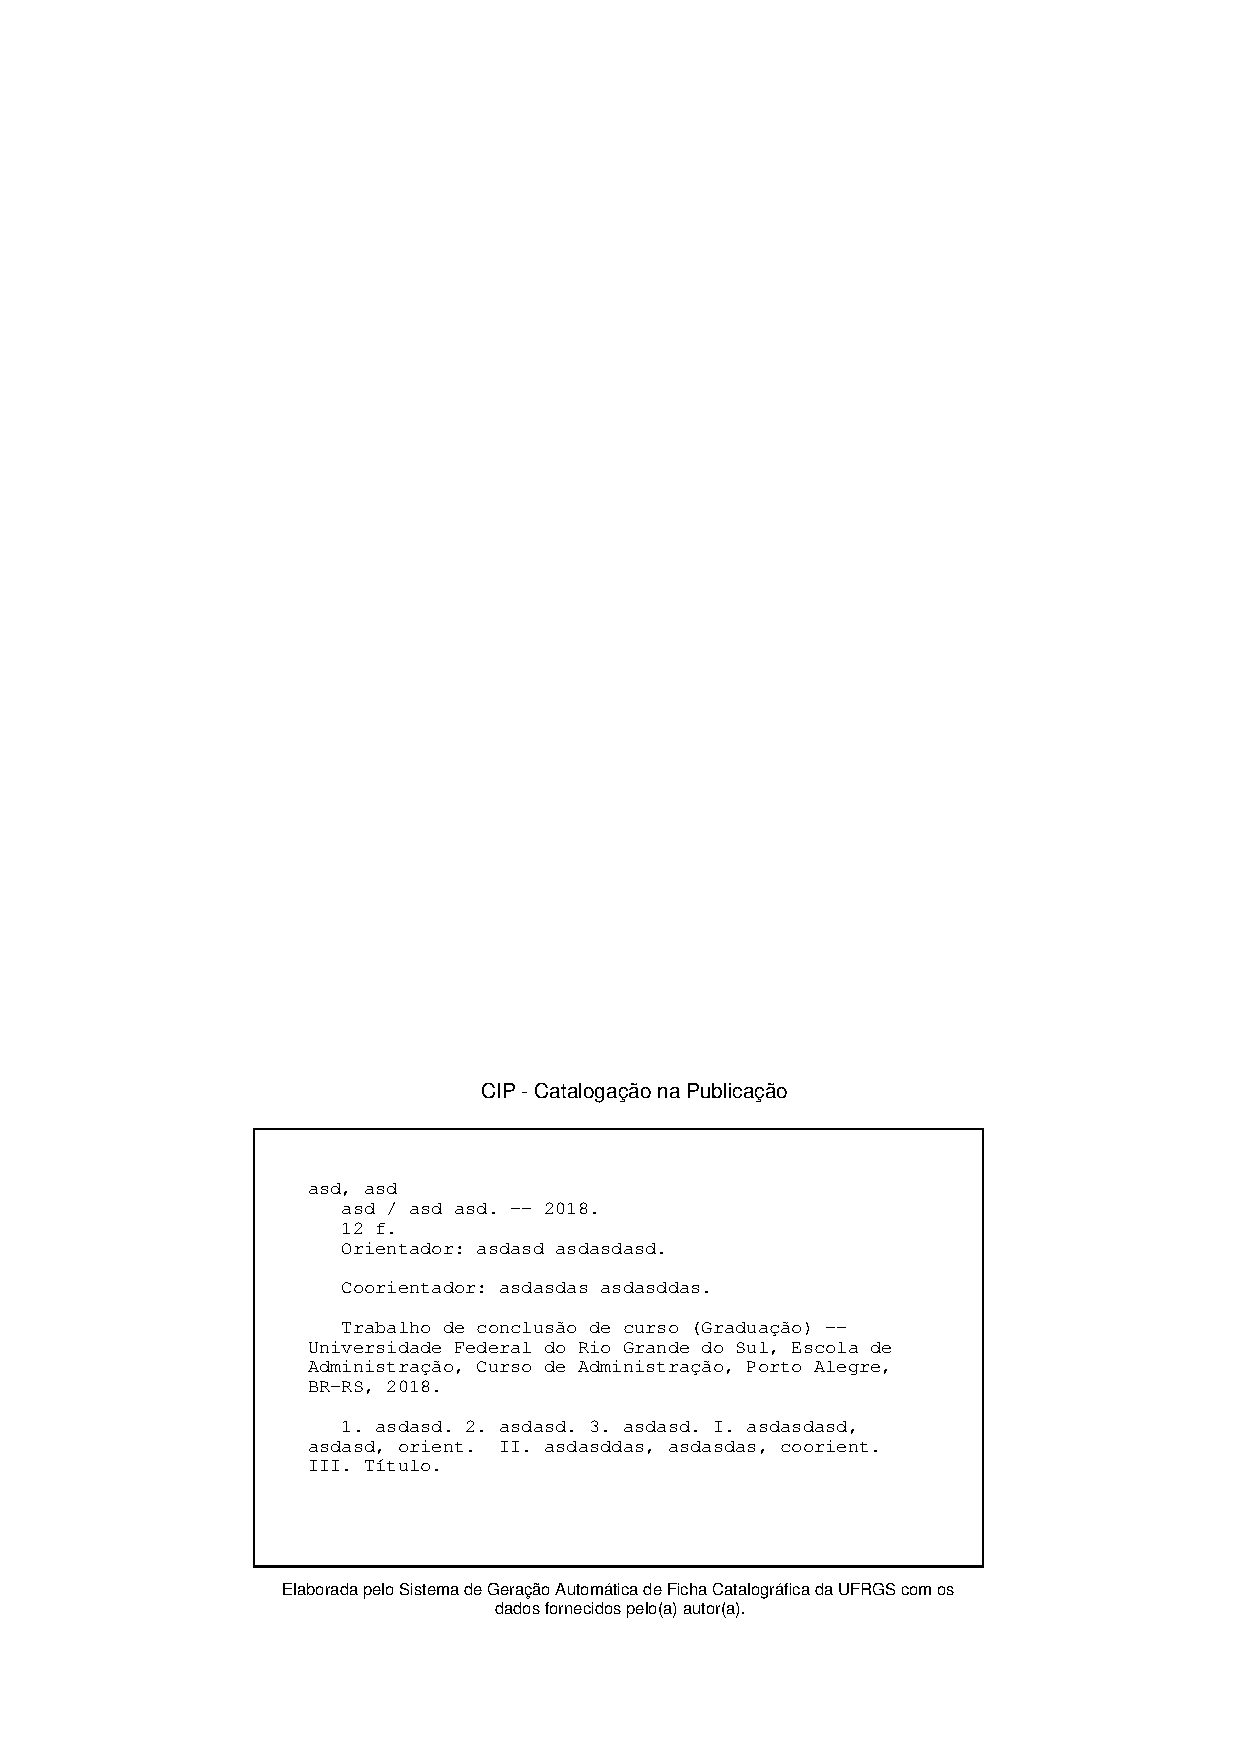
\includepdf[pages=-]{Includes/ficha.pdf}
\end{fichacatalografica}

% ----------------------------------------------------------
% ERRATA
% ----------------------------------------------------------
%\begin{errata}
%Elemento opcional da \citeonline[4.2.1.2]{NBR14724:2011}. Exemplo:

%Se não for usar, deixe o input no "main" comentado  

\vspace{\onelineskip}

FERRIGNO, C. R. A. \textbf{Tratamento de neoplasias ósseas apendiculares com
reimplantação de enxerto ósseo autólogo autoclavado associado ao plasma
rico em plaquetas}: estudo crítico na cirurgia de preservação de membro em
cães. 2011. 128 f. Tese (Livre-Docência) - Faculdade de Medicina Veterinária e
Zootecnia, Universidade de São Paulo, São Paulo, 2011.

\begin{table}[htb]
\center
\footnotesize
\begin{tabular}{|p{1.4cm}|p{1cm}|p{3cm}|p{3cm}|}
  \hline
   \textbf{Folha} & \textbf{Linha}  & \textbf{Onde se lê}  & \textbf{Leia-se}  \\
    \hline
    1 & 10 & auto-conclavo & autoconclavo\\
   \hline
\end{tabular}
\end{table}

\end{errata}
% ---

% ----------------------------------------------------------
% FOLHA DE APROVACAO/QUALIFICACAO
% ----------------------------------------------------------
% % Folha de aprovação
\begin{folhadeaprovacao}

	%\setlength{\ABNTsignthickness}{0.4pt}
	%\setlength{\ABNTsignwidth}{10cm}
	
	% Informações gerais acerca do trabalho 
	% (nome do autor, título, instituição à qual é submetido e natureza)
	\noindent 
	Dissertação de Mestrado sob o título \textit{ \Titulo } apresentada por \textbf{ \Autor} e aceita pelo Programa de Pós-graduação em Sistemas e Computação do Departamento de Informática e Matemática Aplicada da Universidade Federal do Rio Grande do Norte, sendo aprovada por todos os membros da banca examinadora abaixo especificada:
		
	% Membros da banca examinadora e respectivas filiações
\begin{center}
    \assinatura
	{
		{\Orientador}\\
        {\small Orientador}	\\
		{\footnotesize
			\mbox{Departamento de Informática e Matemática Aplicada}\\ 
		  	\mbox{Universidade Federal do Rio Grande do Norte}
		}
   }
\end{center}
\begin{center}
    \assinatura
	{
		Título e nome do professor  			                  \\
		{\small Examinador}											          \smallskip\\ 
		{\footnotesize
			SIGLA -- Institutição		   \\
		  	SIGLA -- Institutição
		}
   }   
\end{center}
\begin{center}
    \assinatura
	{
		Título e nome do professor  			                  \\
		{\small Examinador}											          \smallskip\\ 
	    {\footnotesize
			SIGLA -- Institutição		   \\
		  	SIGLA -- Institutição
		}
	}
\end{center}
\begin{center}
    \assinatura
	{
		Título e nome do professor  			                  \\
		{\small Examinador}											          \smallskip\\ 
		{\footnotesize
			SIGLA -- Institutição		   \\
		  	SIGLA -- Institutição
		}
	}
\end{center} 
	\vfill
	
	\begin{center}
		Cidade-Estado, 01 de janeiro de 1915.
	\end{center}
\end{folhadeaprovacao}


\begin{folhadeaprovacao}

  \begin{center}
    {\ABNTEXchapterfont\large\imprimirautor}

    \vspace*{\fill}\vspace*{\fill}
    \begin{center}
      \ABNTEXchapterfont\bfseries\Large\imprimirtitulo
    \end{center}
    \vspace*{\fill}
    
    \hspace{.45\textwidth}
    \begin{minipage}{.5\textwidth}
        \imprimirpreambulo
    \end{minipage}%
    \vspace*{\fill}
   \end{center}
        
   Trabalho aprovado. \imprimirlocal, 01 de janeiro de 1915:

   \assinatura{\textbf{\imprimirorientador} \\ Orientador} 
   \assinatura{\textbf{título e nome do professor} \\ Examinador}
   \assinatura{\textbf{título e nome do professor} \\ Examinador}
   \assinatura{\textbf{título e nome do professor} \\ Examinador}
   %\assinatura{\textbf{Professor} \\ Convidado 4}
      
   \begin{center}
    \vspace*{0.5cm}
    {\large\imprimirlocal}
    \par
    {\large\imprimirdata}
    \vspace*{1cm}
  \end{center}
  
\end{folhadeaprovacao}

% Folha de qualificacao
% \begin{folhaqualificacao}



	%\setlength{\ABNTsignthickness}{0.4pt}
	%\setlength{\ABNTsignwidth}{10cm}
	
	% Informações gerais acerca do trabalho 
	% (nome do autor, título, instituição à qual é submetido e natureza)
	\noindent 
	Qualificação de Mestrado sob o título \textit{ \Titulo } apresentada por \Autor{} e aceita pelo Programa de Pós-graduação em Sistemas e Computação do Departamento de Informática e Matemática Aplicada da Universidade Federal do Rio Grande do Norte, sendo aprovada por todos os membros da banca examinadora abaixo especificada:
		
	% Membros da banca examinadora e respectivas filiações
\begin{center}
    \assinatura
	{
		{\Orientador}\\
        {\small Orientador}	\\
		{\footnotesize
			\mbox{Departamento de Informática e Matemática Aplicada}\\ 
		  	\mbox{Universidade Federal do Rio Grande do Norte}
		}
   }
\end{center}
\begin{center}
    \assinatura
	{
		Título e nome do professor  			                  \\
		{\small Examinador}											          \smallskip\\ 
		{\footnotesize
			SIGLA -- Institutição		   \\
		  	SIGLA -- Institutição
		}
   }   
\end{center}
\begin{center}
    \assinatura
	{
		Título e nome do professor  			                  \\
		{\small Examinador}											          \smallskip\\ 
	    {\footnotesize
			SIGLA -- Institutição		   \\
		  	SIGLA -- Institutição
		}
	}
\end{center}
\begin{center}
    \assinatura
	{
		Título e nome do professor  			                  \\
		{\small Examinador}											          \smallskip\\ 
		{\footnotesize
			SIGLA -- Institutição		   \\
		  	SIGLA -- Institutição
		}
	}
\end{center} 
	\vfill
	
	\begin{center}
		\Local{}, \DataDaAprovacao{}
	\end{center}
% \end{folhaqualificacao}




% ----------------------------------------------------------
% DEDICATORIA
% ----------------------------------------------------------
% Dedicatória

\chapter*{}
\vspace{15cm}
\begin{flushright}
	Texto de dedicatória. asdasdasdasdas
\end{flushright}


% ----------------------------------------------------------
% AGRADECIMENTOS
% ----------------------------------------------------------
% Agradecimentos
\chapter*{Agradecimentos}

Agradeça a quem você desejar e da forma que você desejar. Este espaço pertence ao aluno e deve ter sua livre expressão de gratidão a quem desejar.

% ----------------------------------------------------------
% EPIGRAFE
% ----------------------------------------------------------
% Epígrafe (citação seguida de indicação de autoria)

\chapter*{}
\vspace{15cm}
\begin{flushright}
	\textit	{
		“Not all those who wander are lost.”
	}\medskip\\ 
	J. R. R. Tolkien
\end{flushright}

% ----------------------------------------------------------
% RESUMO
% ----------------------------------------------------------
\chapter*{}
% Resumo em língua vernácula
\begin{center}
	{\Large{\textbf{\Titulo}}}
\end{center}

\vspace{1cm}

\begin{flushright}
	Autor: \Autor\\
	Orientador: \Orientador
\end{flushright}

\vspace{1cm}

\begin{center}
	\Large{\textsc{\textbf{Resumo}}}
\end{center}

\noindent 
resumo do trabalho em português.


\noindent\textit{Palavras-chave}: palavra\_1; palavra\_2; palavra\_3.






% ----------------------------------------------------------
% RESUMO
% ----------------------------------------------------------
\chapter*{}

% Resumo em língua estrangeira (em inglês Abstract, em espanhol Resumen, em francês Résumé)
\begin{center}
	{\Large{\textbf{Research Title in English}}}
\end{center}

\vspace{1cm}

\begin{flushright}
	Author: Aluno da Silva\\
	Supervisor: Título e nome do seu orientador
\end{flushright}

\vspace{1cm}

\begin{center}
	\Large{\textsc{\textbf{Abstract}}}
\end{center}

\noindent Research abstract fully in English.

\noindent\textit{Keyword\_s}: Word\_1; Word2; Word\_n.

% ----------------------------------------------------------
% LISTA DE ILUSTRACOES
% ----------------------------------------------------------
\chapter*{}
% ---
% inserir lista de ilustrações
% ---
\pdfbookmark[0]{\listfigurename}{lof}
\listoffigures*
\cleardoublepage
% ---




% ----------------------------------------------------------
% LISTA DE TABELAS
% ----------------------------------------------------------
% ---
% inserir lista de tabelas
% ---
\pdfbookmark[0]{\listtablename}{lot}
\listoftables*
\cleardoublepage
% ---

% ----------------------------------------------------------
% LISTA DE ABREVIATURAS E SIGLAS
% ----------------------------------------------------------
\chapter*{Lista de Abreviaturas}

\begin{acronym}

\acro{API}{\textit{Application Programming Interface}}      %exemplo
\acro{BTI}{Bacharelado em Tecnologia da Informação}         %exemplo
\acro{SLA}{\textit{Service Level Agreement}}   
\acro{IoT}{\textit{Internet of Things}}   
\acro{RFID}{\textit{Radio Frequency IDentification}}  
\acro{EN}{\textit{Energy-Neutral Operation}}  
\acro{PNO}{\textit{Power-Neutral Operation}}  
\acro{MDP}{\textit{Markov Decision Process}}  
\acro{EHS}{\textit{Energy Harvesting System}} 

\acro{qos}{\textit{Quality of Service}} 



\end{acronym}

% ----------------------------------------------------------
% LISTA DE SIMBOLOS
% ----------------------------------------------------------
%não usei lista de símbolos, consulte o modelo canônico para mais detalhes

% ----------------------------------------------------------
% SUMARIO
% ----------------------------------------------------------

% ---
% inserir o sumario
% ---
%\pdfbookmark[0]{\contentsname}{toc}
\tableofcontents
%\cleardoublepage


% ---

% ----------------------------------------------------------
% ----------------------------------------------------------
% ELEMENTOS TEXTUAIS
% ----------------------------------------------------------
% ----------------------------------------------------------
\textual

% ----------------------------------------------------------
% Introdução - CAPÍTULO 1
% ----------------------------------------------------------
\addcontentsline{toc}{chapter}{Capítulo 1}
% Introdução - vFinal 1.0 - 04-07-2018
\chapter{Introdução}
\label{cap:cap1}

Nos últimos anos, o avanço das tecnologias de comunicação e a miniaturização dos componentes têm impulsionado significativamente o crescimento da Internet das Coisas (\acl{IoT} - \acs{IoT}). Seus dispositivos estão sendo incorporados em diversas áreas, desde residências inteligentes até cidades conectadas, transformando a forma como interagimos com o mundo ao redor. Esses dispositivos \acs{IoT}, porém, enfrentam um desafio crítico: a eficiência de uso dos recursos energéticos. Disponibilidade e  conectividade constante exigem soluções inovadoras para a gestão de energia, seus esforços resultaram no desenvolvimento de dispositivos sob novo paradigma, os sistemas dirigidos à energia (\acl{EDC}), conceito apresentado por \citeonline{merrett_energy-driven_2017} .

A possibilidade de extração energética de fontes de energia sustentáveis através dos sistemas de coleta (\acl{EHS}), permitiu aos dispositivos responderem às questões inerentes a manter-se operacional mesmo em cenários de intermitência no fornecimento de energia. As soluções comumente passam por utilizar um mecanismo intermediário capaz de armazenar energia com intenção de utilizar esse valor como suplemento nos cenários de variação da performance da coleta \cite{kansal_power_2007}.

Embora dispositivos \acs{IoT} alimentados por um armazenamento energético sejam adequados para muitas aplicações, suas vidas úteis são limitadas pela capacidade fixa do componente embarcado \cite{sliper_energy-driven_2020}. Desafios atuais para estes dispositivos estão intrinsecamente ligados à pratica recorrente do uso de baterias como componente de armazenamento energético. Aspectos sobre o uso destes componentes, estão negativamente relacionados com custo, volume, impacto ambiental, descarte, reciclagem e vida útil dos componentes e redirecionam os esforços em busca por soluções alinhadas à sustentabilidade como visto em \citeonline{albreem_green_2017}.

Sistemas dirigidos à energia são projetados para otimizar o consumo energético, possibilitando sua operação por longos períodos mesmo com recursos limitados. Esses sistemas incorporam diversas características distintivas que os tornam essenciais no ecossistema \acs{IoT}. Estes dispositivos não são projetados apenas considerando as necessidades da aplicação, mas também levam em conta o ambiente e as características energéticas impostas em resposta a desafio energético aplicado. 

Por meio disso, é possível projetar dispositivos com capacidade de operar mesmo em cenários de intermitência no fornecimento energético, reduzindo a necessidade de componentes de armazenamento e, em alguns casos, até mesmo dispensando sua utilização. Sistemas intermitentes \acs{ICS} são projetados não sob a perspectiva de evitar falhas energéticas, mas como os dispositivos podem atuar aceitando a possibilidade de intermitência energética \citeonline{sliper_energy-driven_2020}.

Ademais, é observado os esforços relacionados à maneira como os dispositivos alinham seu comportamento com as demandas operacionais e o fornecimento energético. Este equilíbrio entre disponibilidade e a necessidade de energia é fundamental para garantir o funcionamento eficiente e confiável dos dispositivos \acs{IoT} com restrições energéticas.

Ao combinar essas características, os sistemas dirigidos à energia concentram esforços para que os dispositivos operem de forma eficiente e sustentável, atendendo às exigências de uma ampla gama de aplicações. Desde demandas relacionadas à saúde até automação industrial, a eficiência energética proporcionada por esses sistemas é essencial para a viabilidade e o sucesso da IoT em larga escala \cite{asghari_internet_2019}.


\section{Justificativa}

Dispositivos projetados segundo computação dirigida à energia, precisam garantir certa disponibilidade à medida que adequa-se ao cenário energeticamente restrito. No entanto, alcançar disponibilidade nestes cenários representa desafios consideráveis \cite{sudevalayam_energy_2011}, especialmente quando se trata de dispositivos que dependem da coleta e gerenciamento eficiente de recursos energéticos . 

Neste contexto, a estratégia para manter-se energeticamente disponível passa pela prática de restrição da performance como visto em \citeonline{khairnar_discrete-rate_2015}; \citeonline{doumenis_lightweight_2022}; \citeonline{gong_sleep_2022}. A prática se baseia em reduzir o potencial de consumo energético do dispositivo através da restrição de atividades ou performance, adequando-se ao cenário encontrado. 

Quanto a eficiência sobre o consumo energético, as soluções concentram-se especificamente em seu cenário de aplicação observado. Muito em decorrência do que \citeonline{sliper_energy-driven_2020} escreveu. No seu estudo, o autor chama atenção para a aplicabilidade dos modos de operação: intermitente, neutro-potência e neutro-energética, que, embora tratem sobre aspectos energéticos, divergem por exemplo, no entendimento sobre a presença de um componente auxiliar de armazenamento energético, impactando na definição de quais aspectos considerar para implementar um mecanismo \textit{Throttling} como ferramenta limitadora, tal qual definido em \cite{burns_designing_nodate}. 

A classificação dos cenários de aplicação é essencial para identificar os elementos mínimos necessários para processo de implementar o mecanismo d\textit{throttling}, considerando as especificidades de cada contexto e os termos para disponibilidade a serem alcançadas.

Além disso, a ausência de outras classificações, dificulta a possibilidade de comparação e análise dos diversos aspectos e abordagens presente nas soluções disponíveis para o desafio do consumo energético eficiente.



\section{Objetivos}

Este trabalho contempla como objetivo geral definir e organizar os aspectos necessários para orientar a aplicação da prática \textit{Throttling} recorrentemente presente dispositivos \acs{IoT} em computação dirigida à energia. Para isto, busca-se:

\begin{itemize}
	\item Classificar os elementos recorrentemente presentes em computação dirigida à energia quanto a prática de \textit{throttling} em busca de disponibilidade do ponto de vista energético;
	\item Orientar o processo de implementação da classificação proposta necessários para prática de restrição \textit{Throttling}. 
\end{itemize}

\section{Metodologia}

Para alcançar os objetivos propostos, foram adotados os seguintes procedimentos metodológicos:
\begin{enumerate}
	
	\item Revisão da Literatura;
	\item Classificação dos elementos presentes na forma de taxonomia;
	\item Atividades para implementação da taxonomia proposta;
	\item Estudo Experimental e Avaliação dos resultados.
\end{enumerate}

A revisão do estado da arte desempenhou um papel fundamental na análise dos trabalhos relacionados à adaptação do comportamento dos dispositivos \acs{IoT} em cenários de restrição energética, especialmente em relação às práticas de limitação de desempenho em busca de disponibilidade energética. 

Uma vez conhecidas as características envolvidas na definição do agente limitador, deu-se início ao processo de sistematização e classificação dos aspectos observados na literatura. A abordagem sistemática foi realizada por meio de uma taxonomia, baseada no guia proposto por \citeonline{usman_taxonomies_2017}. Após a definição do modelo de classificação, foram apresentadas as classes e subclasses que estruturam a taxonomia. Essa construção tem como base os principais aspectos envolvidos na atuação do mecanismo limitador nos dispositivos \acs{IoT} em computação dirigida à energia.


Para avaliar as etapas anteriores, foi executado um estudo experimental preliminar como prova de conceito, o qual permitiu, a partir da instanciação das classes necessárias, observar a viabilidade de implementação enquanto a atuação dos agentes limitantes em diferentes cenários de experimentação é observada. Com isso, espera-se que a taxonomia e as atividades realizadas possam ser utilizadas como apoio ao processo de implementação do mecanismo de throttling em cenários \acs{IoT} dirigidos à energia.


\section{Organização da Dissertação }

\begin{comment}
\section{Introduction}
Nos últimos anos, o avanço das tecnologias de comunicação e a miniaturização dos componentes têm impulsionado significativamente o crescimento da Internet das Coisas IoT. Seus dispositivos estão sendo incorporados em diversas áreas, desde residências inteligentes até cidades conectadas, transformando a forma como interagimos com o mundo ao redor. Esses dispositivos (IoT),  enfrentam um desafio crítico: adequar sua operação em detrimento da eficiência de uso dos recursos energéticos. Disponibilidade e conectividade constante exigem soluções inovadoras para a gestão de energia, seus esforços resultam no desenvolvimento de novos dispositivos orientados sob paradigma Energy-Driven Computing \cite{merrett_energy-driven_2017}.

Embora dispositivos IoT alimentados por um armazenamento energético sejam adequados para muitas aplicações, suas vidas úteis são limitadas pela capacidade fixa do componente embarcado \cite{sliper_energy-driven_2020}. É preciso considerar alguns fatores sobre o uso de componentes de armazenamento energético, pois, são negativamente relacionados quanto à custo, volume, impacto ambiental, descarte, reciclagem e vida útil dos componentes e redirecionam os esforços em busca por soluções alinhadas à sustentabilidade \cite{albreem_green_2017}.

Sistemas dirigidos à energia são projetados para otimizar o consumo energético, possibilitando sua operação por longos períodos mesmo em condições limitadas. Esses sistemas incorporam diversas características essenciais para o ecossistema IoT, uma vez que estes dispositivos não são projetados apenas considerando as necessidades da aplicação, mas também levam em conta o ambiente e características energéticas impostas ao desafio de manter os dispositivos operando\cite{sliper_energy-driven_2020}.

Ao combinar essas características, os dispositivos IoT dirigidos à energia concentram esforços para que permaneçam funcionais mesmo em condições restritas, atendendo às exigências de uma ampla gama de aplicações como as relacionadas à saúde até automação industrial \cite{asghari_internet_2019}, a eficiência energética proporcionada por dispositivos desenvolvidos nesse paradigma é essencial para a viabilidade e o sucesso da IoT em larga escala, especialmente em cenários restritos.

Assim, a estratégia para manter-se energeticamente disponível passa pela prática de restrição da performance \cite{khairnar_discrete-rate_2015},\cite{doumenis_lightweight_2022}, \cite{gong_sleep_2022}. Este processo baseia em reduzir o potencial de consumo energético do dispositivo através da restrição de atividades, transmissão ou performance, adequando-se ao cenário encontrado. 

Diante desse desafio, emerge o mecanismo throttling já conhecido em sistemas distribuídos \cite{burns_designing_nodate}, uma prática em busca de responder aos processos necessários para que os dispositivos consigam aplicar suas restrições necessárias enquanto buscam manter-se energeticamente disponíveis. Para isso, é preciso analisar quais os aspectos voltados para estes dispositivos dirigidos à energia são necessários observar para adoção do mecanismo limitador. 

Finalmente, por meio da categorização taxonômica \cite{usman_taxonomies_2017} é possível elencar os atores envolvidos no processo de implementação dos mecanismos limitadores nestes dispositivos dirigidos à energia.

Assim, a taxonomia proposta neste trabalho busca categorizar o conhecimento auxiliando na compreensão dos conceitos relacionados ao escopo que se define um dispositivo IoT em computação dirigida à energia e da aplicação das práticas Throttling como agente colaborador no processo de ajuste de características dos dispositivos em detrimento dos aspectos ligados à disponibilidade.
\end{comment}

% ----------------------------------------------------------
% CAPÍTULO 2
% ----------------------------------------------------------
\addcontentsline{toc}{chapter}{Capítulo 2}
% Capítulo 2 - vFinal 1.0 - 05/07/2018
\chapter{Conceitos Relacionados}
\label{cap:cap2}

Este capítulo aborda os conceitos e técnicas que proporcionam a compreensão dos capítulos a seguir. Na Seção \ref{cap2:iot}, apresento a visão geral sobre Redes IoT e dispositivos que compõe o alvo das iniciativas propostas. A Seção \ref{cap2:energyDriven} introduz o conceito da computação dirigida aos fatores energéticos, tema originador do trabalho.  Por sua vez, na Seção \ref{cap2:throttling} encontram-se os conceitos ligados ao padrão throttling, seus objetivos e aplicação. A intenção de uso de um modelo taxonômico esta fundamentada na Seção \ref{cap2:taxonomia}. Ao fim, na Seção \ref{cap2:consideracoesFinais} estão descritas as considerações ao capítulo.


\section{Internet das Coisas}
\label{cap2:iot}

O termo IoT - Internet das Coisas (\textit{Internet of Things}), foi proposto inicialmente por \citeauthor{ashton1999internet} (\citeyear{ashton1999internet}), e descreve a capacidade de objetos físicos estarem interconectados por meio da internet, viabilizando seus processos de coleta e compartilhamento de dados. Atualmente, a quantidade de dispositivos interconectados cresce diariamente em números impressionantes \cite{lund2014worldwide} uma breve observação da vida diária comprova que nunca tivemos tantos dispositivos inteligentes ao nosso redor, com diversas projeções sendo criadas a respeito da quantidade de elementos interconectados.

Possibilitando a comunicação entre dispositivos,  redes inteligentes podem ser controladas remotamente e automatizadas para realizar tarefas específicas. Essas características favorecem uma variedade de aplicações, incluindo monitoramento, gerenciamento de recursos, saúde digital, cidades inteligentes, agricultura de precisão, e o desenvolvimento de novas aplicações \cite{miorandi2012internet, asghari_internet_2019}.

No entanto, com essa capacidade aprimorada, novos desafios são encontrados à medida que novas aplicações aproveitam suas potencialidades, resultando em soluções mais amplas e aprimoradas a passo que crescem em complexidade. Por exemplo, o aumento do numero de dispositivos interconectados exige uma abordagem mais sofisticada para gerenciamento e segurança em decorrência da massiva quantidade de dados gerados e compartilhados, em paralelo, a interoperabilidade dos sistemas atingem maior importância a medida que o ecossistema das Redes IoT se expande. 

Na revisão proposta em \cite{asghari_internet_2019}, podemos caracterizar os elementos presentes na \acs{IoT}, e, entre outros fatores, de acordo com as seguintes capacidades:

\begin{enumerate}
	%self-adapting
	\item Capacidade de auto-adaptação: Dispositivos e sistemas IoT precisam ser capazes de dinamicamente adaptar-se mudando seu contexto e tomando ações motivadas nas suas condições de operação e contexto de uso. Considerando um sistema de monitoramento de ambientes com câmeras, estas podem adaptar seu modo de operação (com e sem iluminação suficiente) baseando se está de dia ou noite \cite{doumenis_lightweight_2022}. 
	
	%self-configure
	\item Capacidade de auto-configuração: Dispositivos carregam a capacidade de auto configuração, permitindo que dispositivos atuem em conjunto para prover alguma funcionalidade. Estes podem configurar a si mesmo (associado a infraestrutura provida).
	
	%Interoperability
	\item interoperabilidade entre protocolos: Dispositivos IoT podem suportar diversos protocolos de comunicação com outros elementos e infraestrutura.
	
	%Context-awareness
	\item Consciência de Contexto: Uma vez imerso no meio físico, dispositivos podem adquirir conhecimento a respeito das características que o cerca. As decisões tomadas posteriormente podem levar em consideração esses aspectos \cite{yang2014health}.
\end{enumerate}

Neste quesito, os aspectos ligados aos fatores energéticos também se destacam, sobretudo quando estão relacionados aos desafios de manter dispositivos operando eficientemente e de maneira sustentável \cite{albreem_green_2017}. Questões ligadas a eficiência energética, autonomia e a busca de fontes alternativas de suprimento energético bem como a capacidade dos dispositivos em lidar com tais fatores são pontos fundamentais a se pensar. 

Restrições energéticas permanecem como um dos principais temas, desafio que afeta a performance e disponibilidade de elementos nas redes IoT. Atualmente, as soluções mais promissoras para tal são os esforços na gerencia de energia \cite{singh_survey_2020}. Em alguns cenários, a solução mais adequada para estas questões passa pela ação de coletar energia do meio onde o dispositivo esta inserido. Segundo \cite{kansal_power_2007}, um \ac{EHS} ou Sistema de Coleta Energética é o dado sistema complexo capaz de captar energia do ambiente que se encontram convertendo para seu uso.

Desde modo, dispositivos encontrados em tal cenário carregam em suas características fundamentais a necessidade de lidar com os aspectos energéticos, como proposto por \citeauthor{kansal_power_2007} (\citeyear{kansal_power_2007}). Sobretudo com a capacidade de coleta energética, algumas estratégias podem ser tomadas com base nas características embarcadas nos dispositivos, pois em tal cenário precisam ser projetados com a capacidade de autoadaptação, permitindo ajustar-se dinamicamente em acordo com as condições encontradas, demandas operacionais e oferta energética. A consciência de contexto aqui permite a eles compreender e responder às mudanças no ambiente circundante, adaptando-se ou reconfigurando-se proativamente para operar adequadamente frente as condições encontradas. Essas capacidades combinadas com seu sistema de coleta de energia habilita que dispositivos IoT possam gerenciar seus aspectos energéticos de maneira inteligente e responsiva, otimizando seu desempenho enquanto minimizam o consumo de energia buscando perpetuar-se disponível, desde que projetado para tal, contribuindo sobretudo para eficiência geral dos sistemas IoT.



%desafios energéticos para IoT

%areas de solução

\section{\textit{Energy-Driven Computing}}
\label{cap2:energyDriven}

Um sistema dirigido à energia (\textit{Energy-Driven}) é todo aquele que os fatores energéticos intrínsecos a ele são tratados como primários, desde concepção, gerenciamento e sua operação \cite{merrett_energy-driven_2017}. Computação dirigida a estes fatores, ditos energéticos, deve considerar fundamentalmente a disponibilidade energética pois precisam carregar a capacidade de adaptação as dinâmicas de captação de energia. Este paradigma tem como objetivo evidenciar as características energéticas, em potencial a respeito de dispositivos que por quaisquer motivos, não podem estar conectados diretamente em uma infraestrutura capaz de fornecer energia virtualmente ilimitada. 

Para tal, caso necessário, dispositivos podem operar coletando recursos disponíveis no ambiente. Coleta de energia refere-se a capacidade de um dispositivo em capturar e converter recursos energéticos do meio e converte-los de modo a prolongar sua vida útil mitigando um cenário de escassez energética \cite{sudevalayam_energy_2011}. 

Ainda, no trabalho de \citeauthor{sliper_energy-driven_2020} (\citeyear{sliper_energy-driven_2020}) é importante destacar como os mecanismos de coleta energética e sua dinâmica são dispostos. É proposto uma organização em três categorias distintas: Neutra-Energética \ac{EN}, Neutra-Força ou Neutra em Consumo \ac{PNO} e por fim, Operações Intermitentes.

\subsection{Operação \textit{Neutra-Energética}}
Uma operação neutra-energética cobre as dinâmicas dos sistemas com coleta de energia do ambiente por meio de um \textit{buffer}, uma bateria recarregável ou super capacitor capaz de armazenar parte da energia coletada \cite{kansal_power_2007}. Este recurso se encontra disposto entre a entrada energética e sua demanda, atuando secundariamente quando a energia disponibilizada não seria suficiente para manter seus critérios de qualidade de serviço \textit{QoS}.

Apesar de inicialmente ser previsto um cenário de uso onde apenas a fonte energética e o dispositivo estivessem presentes, é comum o fato dos mecanismos que buscam esse tipo de operação recorrer a presença deste componente intermediário capaz de armazenar energia e disponibiliza-la para uso. Sendo assim, na Figura \ref{fig:cap2harveststoreuse} temos a visão geral em blocos de um subsistema responsável pelos recursos energéticos.

\begin{figure}[H]
	\centering
	\caption{Diagrama de blocos subsistema energético para operação neutro-energética.}
	\label{fig:cap2harveststoreuse}
	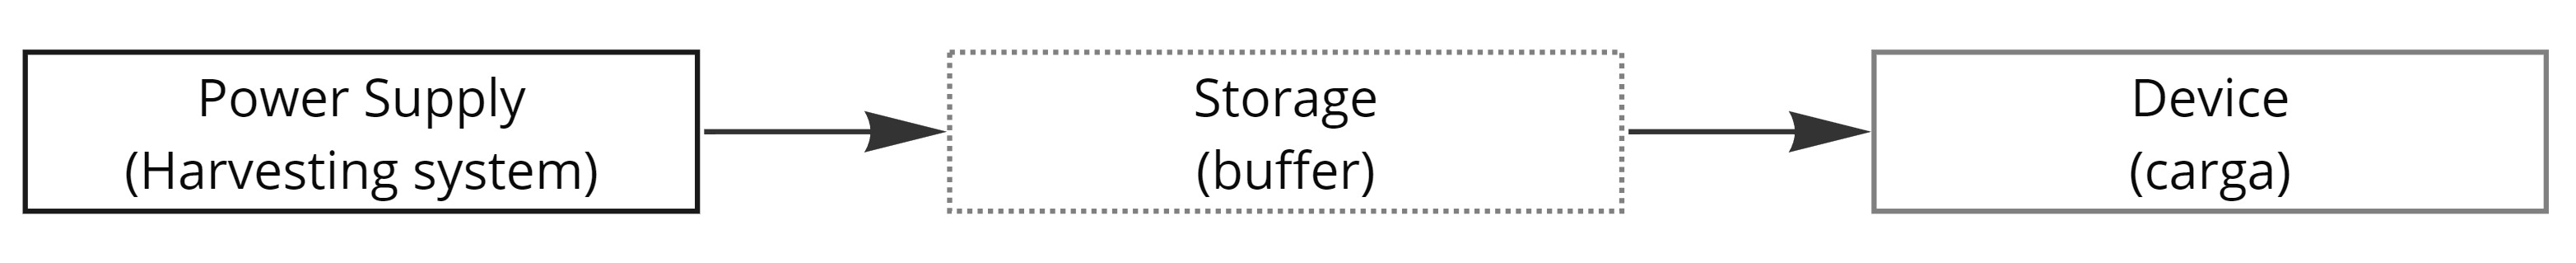
\includegraphics[width=0.7\linewidth]{Imagens/cap2/cap2harvest_store_use}	
	
	Fonte: adaptado de \citeauthor{sudevalayam_energy_2011} (\citeyear{sudevalayam_energy_2011} )
\end{figure}

A visão do cenário acima proporciona ao node a capacidade de manter seus níveis de operação, abstraindo em algum nível as variações de energia coletada. Pois seja $P_{s}(t)$ a entrada energética em dado momento e  $P_{c}(t)$ a energia consumida nos ciclos de carga, é possível encontrar a dinâmica apresentada na Figura \ref{fig:cap2energyneutraloperation}, em momento de abundancia energética o node pode armazenar a energia que supera a quantidade necessária para sua operação em decorrência de que em momentos de escassez, possa fazer uso dessa energia suplementando sua necessidade. 


Operações neutro-energéticas carregam dois princípios que são apresentados no trabalho seminal \cite{kansal_power_2007}: Manter-se operacional mesmo em cenários onde a quantidade de energia coletada fosse durante muito tempo, inferior ao necessário e como garantir que, encontrado em um ambiente de coleta seja possível obter performance esperada tolerando variações da energia coletada. 

\begin{figure}[H]
	\centering
	\caption{Dinâmicas de operação com coleta de energia} \label{fig:dinamicas}
	\begin{subfigure}{0.49\textwidth}
		\caption{Operação com buffer intermediário.}
		\label{fig:cap2energyneutraloperation}
		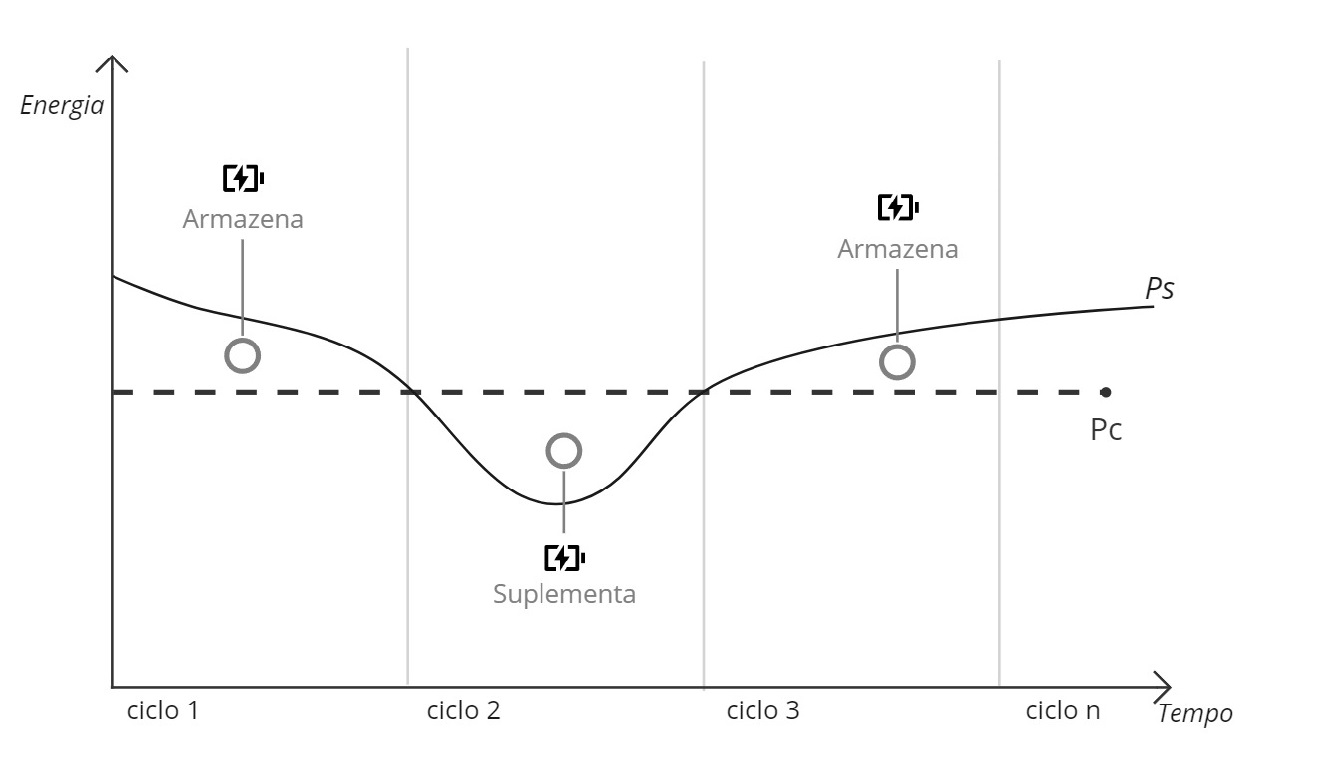
\includegraphics[width=\linewidth]{Imagens/cap2/cap2energyneutraloperation.jpg}	
	\end{subfigure}%
	\hspace*{\fill}  
	\begin{subfigure}{0.49\textwidth}
		\caption{Operação Power-Neutral.}
		\label{fig:cap2powerneutraloperation}
		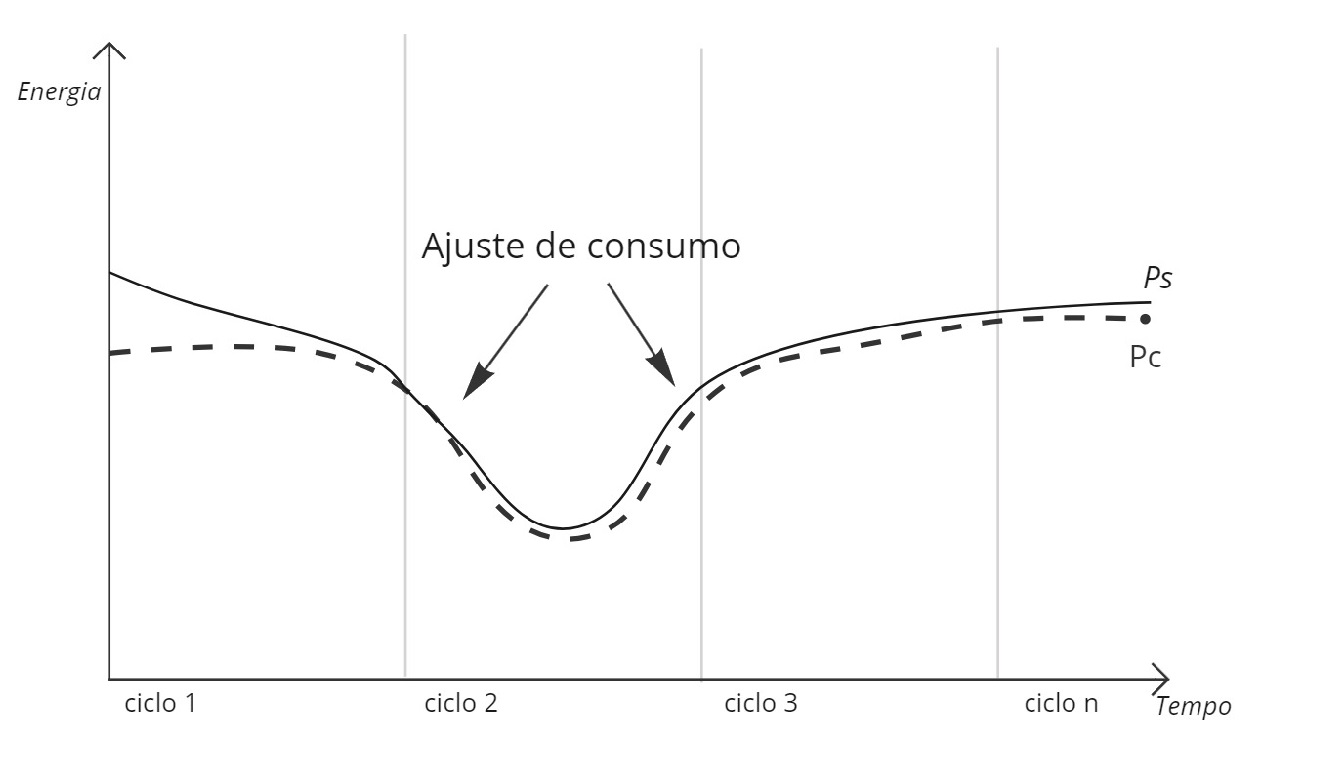
\includegraphics[width=\linewidth]{Imagens/cap2/cap2powerneutraloperation.jpg}
	\end{subfigure}%
	\hspace*{\fill}   
	
	Fonte: elaborado pelo autor.
\end{figure}

Sendo assim, uma operação neutro-energética implica em manter sua a performance durante os ciclos de trabalho garantindo que o node não sofra por esgotamento energético. Busca-se perpetuar sua operação mediante uso da reserva energética ou adaptação motivada a expectativa de recurso futuro \cite{sudevalayam_energy_2011}. Desta forma, o dispositivo favorecido pode prolongar sua operação mesmo em decorrência da indisponibilidade ou insuficiência de fonte energética.

É importante destacar que este modo de operação serviu como base para diversos avanços em computação dirigida a energia sobretudo em redes constituídas tipicamente com sensores embarcados, autônomos e distribuídos espacialmente, \acf{WSN}. Além disso, os conceitos de operação-neutra e a teoria de coleta energética foram fundamentais para o que posteriormente foi detalhado em referencia ao seminal \cite{merrett_energy-driven_2017}, introdutório ao modelo \acf{PNO}.



\subsection{Operação \textit{Power-Neutral}}
A capacidade de um dispositivo em coletar energia do ambiente apresenta diversos desafios, especialmente em relação ao processo de coleta, transformação e uso, bem como à previsibilidade da oferta de energia. A abordagem ilustrada na Figura \ref{fig:cap2harveststoreuse} é típica de um sistema que utiliza um buffer intermediário, com o objetivo de operar semelhante a um sistema tipicamente alimentado por baterias, onde as condições energéticas são resumidas apenas pela condição da reserva energética disponível. No entanto, em muitos casos, os componentes adicionais necessários para garantir essas características aumentam custos, volume e complexidade, podendo resultar em comportamento não confiável se mal projetados.

De acordo com \citeauthor{merrett_energy-driven_2017}(\citeyear{merrett_energy-driven_2017}), os esforços para projetar sistemas com capacidade de coleta de energia devem agora considerar casos onde não é possível incluir um componente de armazenamento energético intermediário. Portanto, os sistemas nessas condições devem buscar o modo intermitente ou mesmo \textit{Power-Neutral}, conforme ilustrado na Figura \ref{fig:cap2powerneutraloperation}.

A Operação \textit{Power-Neutral} envolve adaptar o consumo de energia do dispositivo para manter sua operação de acordo com os recursos disponíveis, minimizando ou até mesmo eliminando a necessidade de armazenamento intermediário de energia \cite{sliper_energy-driven_2020}. No entanto, é importante observar que, se a energia coletada for inferior ao mínimo necessário, o dispositivo entrará em um estado de esgotamento, podendo hibernar caso caracterizado por uma abordagem intermitente \cite{merrett_energy-driven_2017}.



\section{\textit{Throttling}: Padrão de Comportamento em Ambientes Distribuídos}
\label{cap2:throttling}

Como ponto de partida, é preciso destacar a importância da adoção dos ditos padrões \textit{patterns}, especialmente aplicados em sistemas distribuídos. Tais soluções carregam aspectos intrínsecos à experiencia adquirida mediante a recorrência de soluções frente à heterogeneidade de problemas que corrigem, formando o conjunto de atuação onde um ou mais padrões de solução emergem como resposta. Endossado pelo trabalho de \citeauthor{burns_designing_nodate} (\citeyear{burns_designing_nodate}) e no cenário de computação distribuída, é observado que apesar da diversidade de possibilidades para um sistema qualquer, a maneira como é concebido, desenvolvido e por consequência os problemas encontrados sobretudo quanto  aspectos não funcionais como escalabilidade, confiabilidade ou disponibilidade são notavelmente recorrentes e semelhantes. 

O proposito de adotar o padrão Throttling é fazer com que dado sistema alvo mantenha seus níveis de consumo abaixo de um determinado termo, limiar. Assim, conservando seus recursos disponíveis que de outra forma seriam disponibilizados para solicitantes excessivamente demandantes. Além de proteger-se do comportamento inadequado dos agentes envolvidos, é preciso ter em mente que eventualmente um sistema pode encontrar-se tendo de lidar com picos de operações, cenário propício a falhas ou até mesmo interrupção integral do serviços. 

Ambientes IoT representam um domínio onde esse padrão pode ser bastante necessário dado a dinâmica de dispositivos desconhecidos e novos sistemas que podem ser adicionados a um ambiente. Throttling pode ser implementado segundo algumas estratégias elencadas por \citeauthor{martinekuan_throttling_nodate} (\citeyear{martinekuan_throttling_nodate}):

\begin{itemize}
	\item Rejeitando requisições de um agente excessivamente solicitante.
	\item Desabilitando ou degradando componentes ligados a operações menos essenciais. 
	\item Estabelecendo níveis de prioridade para os agentes solicitantes, onde requisições de níveis menos prioritários podem ser suspensas ou limitadas em detrimento de outra com mais privilégio, durante algum tempo, conforme Figura \ref{fig:cap2throttlingexample}.
\end{itemize}

\begin{figure}[H]
	\centering
	\caption{Throttling pode ser aplicado uma vez estabelecidos critérios de prioridade de operações}
	\label{fig:cap2throttlingexample}
	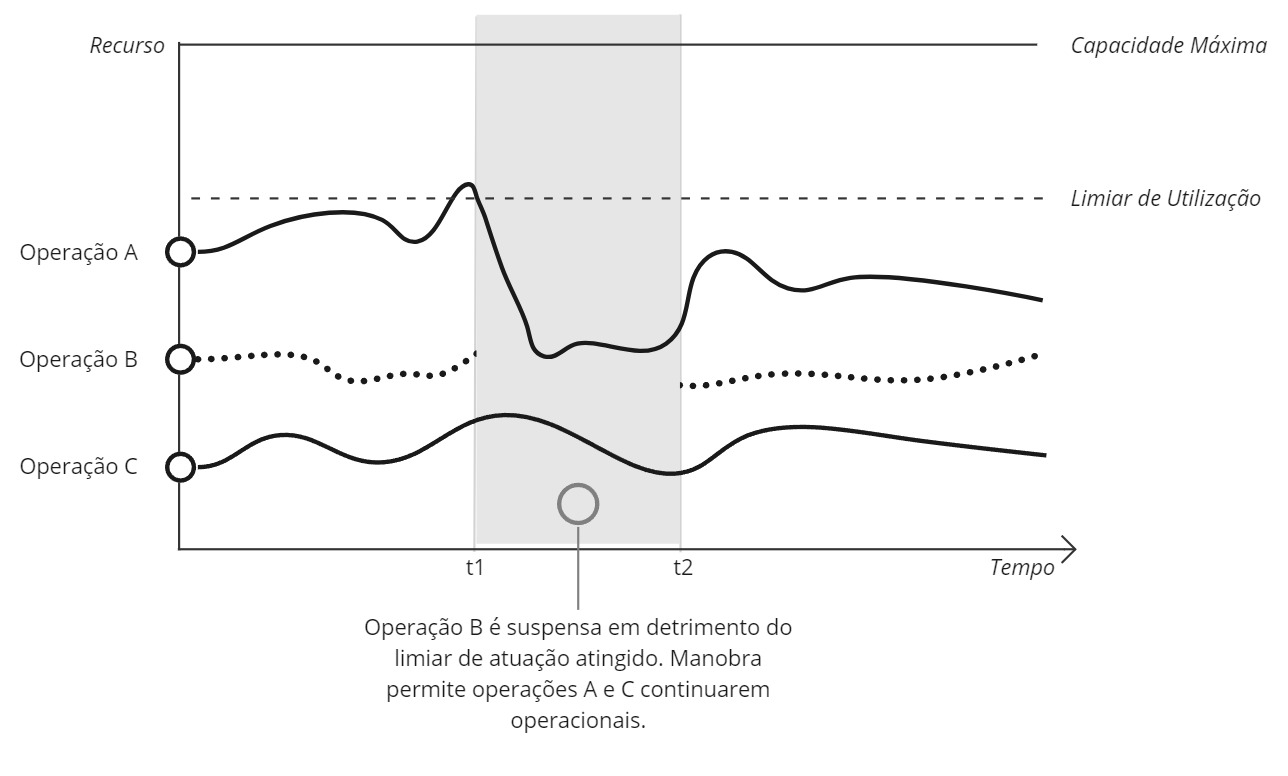
\includegraphics[width=0.7\linewidth]{Imagens/cap2/cap2throttlingexample}	
	
	Fonte: adaptado de \citeauthor{martinekuan_throttling_nodate} (\citeyear{martinekuan_throttling_nodate})
\end{figure}

\subsection{Considerações}
Assim como outros padrões aplicados a sistemas distribuídos, existem uma série de considerações a serem tomadas mediante a decisão de implementar um mecanismo de throttling, \cite{martinekuan_throttling_nodate} aponta alguns tópicos que possibilitam a análise de conformidade face aos problemas e necessidades ao adotar o padrão.  

Utilizar mecanismos de throttling passam por decisões arquiteturais de como o dispositivo vai se comportar. Por isso, deve-se levantar primariamente seu uso nos estágios iniciais de concepção do dispositivo ou sistema.

Um vez estabelecido, caso limiar de atuação seja atingido, os mecanismo de throttling deve ser acionado em conformidade, e uma vez restabelecido ao seu estado regular de atuação, permitir o retorno as capacidades do dispositivo.

É interessante padronizar os retornos dados as solicitações negadas ativamente pela ação do throttling, dando condições do agente solicitante em tomar a melhor decisão entre refazer a solicitação ou aguardar momento oportuno.

Dispositivos capazes de adaptar-se mediante quaisquer fatores devem ter seu comportamento refletido no mecanismo de throttling, preferencialmente em tempo de execução. Eventualmente um cenário onde amparado por uma condição do dispositivo seria tolerado pode não ser mais, o movimento inverso também é valido, condições não toleradas podem passar a ser, mediante evento motivador. 

\section{Taxonomia}
\label{cap2:taxonomia}

Taxonomia refere-se a um sistema de classificação e organização. Seu modelo consiste em sistematicamente apresentar os elementos de um campo de estudo, categorizados e por conseguinte classificados de modo a apresentar os elementos dispostos em estrutura adequada.

O mapeamento sistemático apresentado por \citeauthor{usman_taxonomies_2017} (\citeyear{usman_taxonomies_2017}), trata dos métodos e da aplicação de taxonomias em campos da engenharia de software. O procedimento classificação define como as instâncias de um tema podem ser atribuídos a classes ou categorias. Para uma taxonomia, tais elementos podem estar relacionados e dependentes entre si. Por sua vez, é possível classificar de duas maneiras: Quantitativamente, onde os procedimentos de classificação são baseados em escalas numéricas ou Qualitativa onde uma escala nominal que expresse a categoria será utilizada. Sua estrutura, poderá ser dividida em quatro visões de descobrimento do conhecimento \cite{kwasnik_role_nodate}.

\textbf{Hierárquica}, aqui a taxonomia é estruturada como uma única classe superior (superclasse) que abrange suas subclasses e sequencialmente as possíveis extensões destas, formando um encadeamento hierárquico entre os elementos desde o originário até os derradeiros derivados. Este modelo procura garantir a exclusão mutua entre os envolvidos além do aspecto de relacionamento hereditário, por isso não é recomendado em situações onde uma pesquisa precisa incluir múltiplos e diversos critérios de diferenciação. Por fim, o autor considera que para esta representação é mandatório bom conhecimento sobre o assunto a ser classificado., pois suas classes e critérios de separação precisam ser conhecidos desde o inicio.

\textbf{Árvore} similar ao modelo hierárquico, todavia em uma estrutura árvore não existe um relacionamento do tipo herança. Aqui, o tipo de classificação que busca-se é a relação causa-efeito, processo-produto ou parte-todo. Pode-se usar a estrutura arvore para mostrar a decomposição de um tema em seus aspectos. Por exemplo, a representação em árvore parte-todo do relacionamento entre um país, seus estados e por fim, municípios. Estruturas árvores e hierárquicas compartilham das mesmas limitações.

\textbf{Paradigma}, conduz a taxonomia para a capacidade de um relacionamento bi-direcional entre as classes estas, por sua vez, podem ser descritas pela combinação de dois atributos. Uma proposta de visualização para taxonomias desse tipo é a capacidade de expressar-se com matrizes bi-dimensionais cujo seus vértices apresentam os atributos de interesse.

\textbf{Facetada}, esta estrutura taxonômica permite observar os assuntos classificados sob múltiplas perspectivas (facetas). O indicador fundamental em utilizar uma análise facetada é a necessidade de visualizar mais de uma perspectiva de uma entidade complexa. Cada faceta é independente e pode ter suas próprias classes, permitindo a evolução de cada uma dentro da sua perspectiva. Análise facetada é adequada para campos de conhecimento relativamente novos em constante evolução, dado que não é necessário ter o completo conhecimento do objeto de estudo. Em todo caso, pode ser desafiador encontrar o conjunto inicial de facetas para a taxonomia de modo que sejam independentes e sem aparente relacionamento significativo entre as facetas.

Em \cite{smite_empirically_2014}, o autor indica três mecanismos como validadores de uma taxonomia: a demonstração ortogonal de perpendicularidade e dimensões das classes é demonstrada; análise de desempenho (\textit{Benchmarking}), em que a taxonomia pode ser comparada com outros esquemas de classificação similares; e, por fim, a demonstração de utilidade, validada por estudo de caso ou experimentação.

O entendimento sobre qual visão utilizada para construção de uma taxonomia é crucial, pois impacta diretamente na sobre a maneira como representar classes e interações. Quanto à aplicação prática para Engenharia de Software, ao adotar o uso de uma taxonomia proporciona os agentes facilitadores para atividades de classificar e organizar o conhecimento de uma determinada área \cite{usman_taxonomies_2017}, auxiliando no desdobramento do objeto de estudo, elucidação e identificação de oportunidades e trabalhos futuros.

\section{Considerações Finais}
 \label{cap2:consideracoesFinais}
 
 Neste capítulo foram apresentado os conceitos relacionados que indicam o apoio teórico necessário para a construção do trabalho. Assim, a Seção \ref{cap2:iot} apresenta uma introdução à IoT em destaque para relação com a problemática das restrições energéticas e os mecanismos de coleta energética. A seguir, na Seção \ref{cap2:energyDriven} são descritos os principais modos de operação para computação dirigida a energia \textit{Energy-Drive Computing}. Posteriormente, Seção \ref{cap2:throttling} trás o agente motivador para uso de padrões utilizados em sistemas distribuídos, em especifico Throttling, como um artefato adequado para controle de comportamento dos dispositivos mediante mudança de contexto. Por último, a Seção \ref{cap2:Taxonomia} destacou os propósitos de uma taxonomia e explicou como essa abordagem pode ser útil para organizar um conhecimento e identificar áreas de pesquisa importantes.


% ----------------------------------------------------------
% CAPÍTULO 3
% ----------------------------------------------------------
\addcontentsline{toc}{chapter}{Capítulo 3}
% Capítulo 3
\chapter{Revisão do Estado da Arte}
\label{cap:cap3}

Este capítulo busca compreender o estado da arte e identificar desafios e oportunidades de pesquisa sobre a implementação de mecanismo \textit{throttling}, especialmente no contexto de dispositivos \acs{IoT} presentes na computação dirigia à energia (\acl{EDC}). Assim, foi realizado uma pesquisa sobre a aplicação de fatores limitantes e os motivadores da atuação desse mecanismo.


\section{Protocolo}
Para esta revisão, adotaram-se práticas descritas no método apresentado por \citeauthor{kitchenham_systematic_2009} (\citeyear{kitchenham_systematic_2009}), mas decidiu-se por não utilizar uma revisão sistemática como protocolo. Assim, a captação dos estudos foi realizada através da aplicação da técnica de \textit{snowballing}, que é capaz de expandir a base de referências e viabilizar a identificação de padrões recorrentes, aprofundando a compreensão no tema de estudo.

O processo de \textit{snowballing} é descrito como abordagem iterativa de busca por referências em revisões de literatura \cite{wohlin_guidelines_2014}. Seu método é caracterizado através das iterações onde em cada uma é realizado análise sobre as referencias citadas nos artigos seminais (\textit{backward}) e também dos estudos que utilizaram esses artigos como referencia (\textit{forward}). Portanto, neste trabalho a abordagem de \textit{snowballing} foi executada em iterações, aplicando ambos os métodos (\textit{backward} e \textit{forward}). Os trabalhos resultantes de cada iteração  foram incluídos com base nos critérios de seleção previamente definidos na Subseção \ref{cap3:criteriosinclusaoexclusao}.


\subsection{Critérios de inclusão e exclusão} 
\label{cap3:criteriosinclusaoexclusao}

Tendo em vista a necessidade de realizar filtragem no material encontrado durante iterações, foram adotados critérios de inclusão e exclusão como já previsto no método em  \cite{wohlin_guidelines_2014}. Assim, os estudos resultantes foram obtidos com base nos critérios definidos com a intenção de cobrir o maior numero de trabalhos relacionados ao tema de pesquisa e ao mesmo tempo evitar os trabalhos com base nos critérios estabelecidos.

Portanto, os critérios de exclusão utilizados podem ser vistos descritivamente na Tabela \ref{table:cap3:criterios}. Estes critérios foram definidos para assegurar que apenas os estudos que se relacionassem com a pesquisa fossem incluídos, evitando artigos segundo os critérios ja apresentados.


\begingroup
\begin{table}[htbp]
	
	\centering
	\caption{\textit{Snowballilng}: Critérios de Exclusão.}
	%	\small
	%	\tabcolsep=0.05cm
	\begin{tabular}{ l | l  }
		\hline
		 \multicolumn{2}{c}{Critério de Exclusão}  \\
		\hline\addlinespace[1pt]
		CE-1	& Não escrito em inglês. \\
      	CE-2	& Sem aderência aos eixos temáticos. \\
		CE-3	& Sem indícios diretos com às questões de pesquisa.\\
		CE-4	& Artigos derivações do mesmo autor  ou resumo.\\
		CE-5	& Tutoriais, Capítulos de livros e Relatórios técnicos (Literatura Cinza).\\
		CE-6	& Trabalhos duplicados.\\
		CE-7	& Artigos não disponíveis integralmente para leitura.\\
		CE-8	&  Artigos predecessores à revisão seminal.\\
		\hline\addlinespace[2pt]
	\end{tabular}
	\label{table:cap3:criterios}
	\\
	\footnotesize Fonte: elaborado pelo autor.
	
\end{table}
\endgroup

\subsection{Processo}

Para selecionar os estudos que formam a base do trabalho foi utilizada a base bibliográfica SciVerse Scopus
\footnote{Plataforma acessível em: \url{https://www.scopus.com/}}. A escolha desta plataforma como fonte de informação foi justificada pela capacidade de indexar os principais repositórios acadêmicos para a area de estudo, dentre elas ACM Digital Library, Elsevier, IEEE Xplore, Springer Link, Web of Science entre outras.

O artigo seminal foi selecionado mediante análise de sua influência, impacto e credibilidade para o campo de pesquisa deste estudo. Portanto, utilizando o artigo como único ponto de partida, segue o processo iterativo \textit{snowballing} conforme estabelecido. As etapas podem ser visualizadas na Figura \ref{fig:cap3snowballing} onde é apresentado a visão completa do processo e ações determinadas.


\begin{figure}[H]
	\centering	
	\caption{Processo \textit{Snowballing}.} 
	\label{fig:cap3snowballing}
	\noindent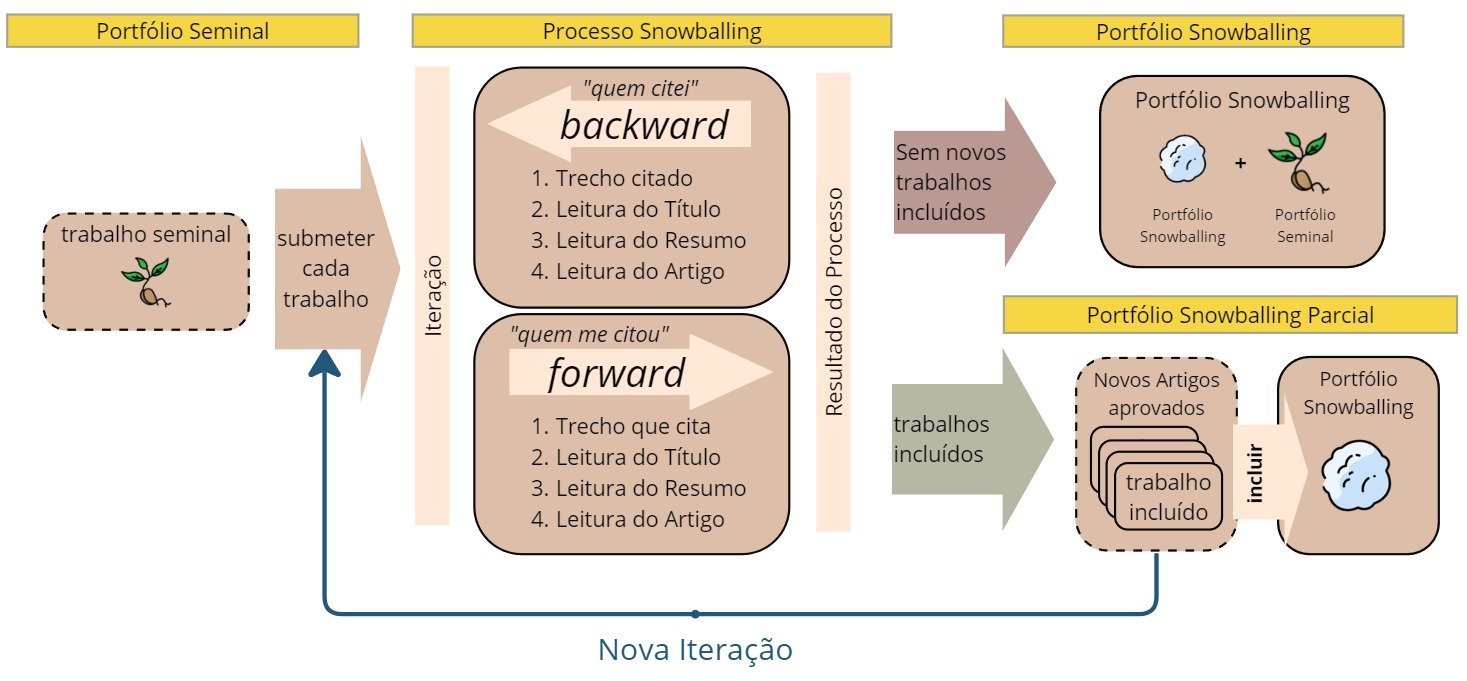
\includegraphics[width=1\linewidth]{Imagens/cap3/snowballing.jpg} 
	
	Fonte: elaborado pelo autor.
\end{figure}

Em cada iteração, são realizadas ações com o objetivo de selecionar os trabalhos considerados relevantes para o estudo. Essas, partem da análise da leitura da parte do texto que foi citado quando em \textit{backward} ou a leitura do trecho que cita quando em \textit{forward}, além da leitura do titulo, resumo e por fim, da leitura integral do trabalho. Assim, ao passo que finalizada interação, teremos os novos artigos que servem como entrada para iteração seguinte. Caso uma iteração finalize sem nenhum novo trabalho adicionado, conclui-se o processo \textit{snowballing}, os resultados são unidos ao artigo seminal em composição ao portfólio final obtido. A Figura \ref{fig:cap3etapassnowballing} apresenta o processo de seleção dos trabalhos avaliados.

\begin{figure}[H]
	\centering	
	\caption{Resultado das Iterações \textit{Snowballing}.} 
	\label{fig:cap3etapassnowballing}
	\noindent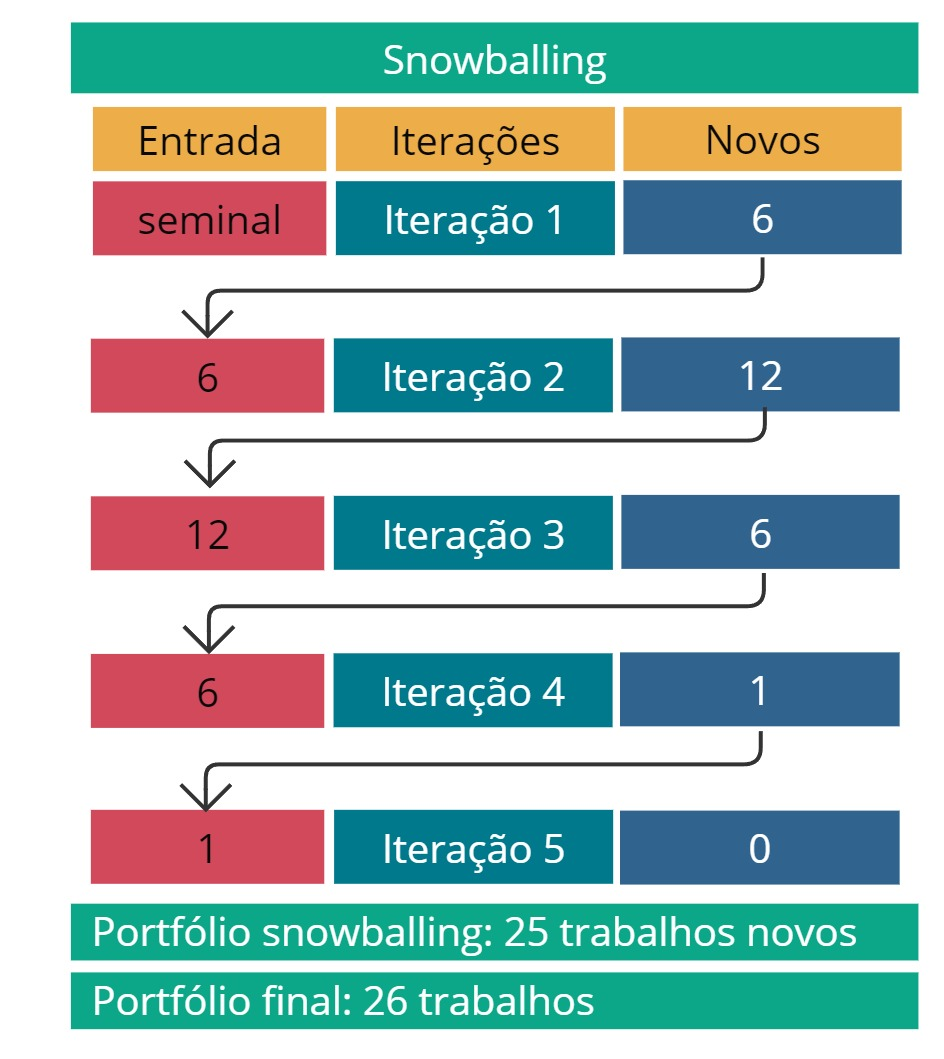
\includegraphics[width=0.7\linewidth]{Imagens/cap3/etapas.jpg} 
	
	Fonte: elaborado pelo autor.
\end{figure}


A dinâmica de inclusão e filtragem de trabalhos relacionados, proporcionou visitar ao todo 1132 trabalhos por método \textit{backward}, além de 3582 trabalhos por \textit{forward} gerando uma cobertura total de 4714 artigos alcançados. É previsto durante o \textit{snowballing} proporcionar rastreabilidade na inclusão dos trabalhos. A Figura apresenta esta característica enquanto proporciona visão sobre os trabalhos mencionados. 

\begin{figure}[H]
	\centering	
	\caption{PENSANDO SE VALE APRESENTAR GRAFO COM A a rastreabilidade dos trabalhos aqui.} 
	\label{fig:cap3etapassnowballing}
	\noindent\includegraphics[width=0.7\linewidth]{example-image} 
	
	Fonte: elaborado pelo autor.
\end{figure}

Finalmente o processo Snowballing proporcionou a criação do portfólio total de artigos, composto por 25 trabalhos que serviram como base para o estudo, os resultados obtidos estão descritos na Seção \ref{cap3:resultados}.


\section{Resultados}
\label{cap3:resultados}

Foi característica do portfólio de trabalhos a apresentação dos desafios enfrentados pelos agentes \acs{IoT} com capacidade de coleta de energia ao realizar suas funções, mesmo diante de restrições energéticas. Nestes trabalhos, foi observada a presença de mecanismos de ajuste do comportamento que utilizam observações de determinadas variáveis para tomar decisões sobre como o dispositivo deve conduzir seus ciclos em diferentes cenários.

Sendo assim, mediante desafios apresentados nos estudos quanto à gestão energética desses dispositivos, foi considerado categorizar dos trabalhos em função dos grupos definidos no estudo \cite{khan_energy_2015}. Por análise de atuação orientada à dados, os trabalhos apresentam a possibilidade de atividades em respeito a previsibilidade dos dados de coleta e demanda energética. Assim, a categorização puramente baseada nos ciclos (\textit{Duty-Cycle}) do dispositivo carregam os fatores de observação atrelados as aspectos energéticos de coleta e armazenamento como motivadores para ajustes no tempo de ciclos ou ocorrência destes para adaptar-se aos critérios de energéticos impostos.

Portanto, diante dos desafios identificados nos estudos sobre a gestão energética desses dispositivos, optou-se por categorizá-los com base nos grupos definidos no estudo realizado por \cite{khan_energy_2015}. Nesse contexto, um grupo de trabalhos se concentram aos desafios de definir os ciclos de operação observando eventos relacionados aos aspectos energéticos de coleta e armazenamento respectivamente. Por sua vez, ao abordar o processo de definir seus ciclos, alguns estudos apontam avanços em tecnicas que buscam prever o comportamento do dispositivo, em especial sua demanda e capacidade de coleta de energia. 

Em última análise, todos os esforços convergem para a análise de como os estudos moldam o escopo decisório da ação do agente limitador (\textit{throttling}) sobre seus ciclos. Além disso, o portfólio alcançado inclui cinco trabalhos categorizados como filosóficos, caracterizados pela apresentação de contribuições puramente conceituais. Esses trabalhos se concentram na análise teórica dos problemas relacionados à computação voltada para a energia, sem necessariamente fornecer implementações práticas, o que se alinha ao modelo de categorização proposto por \citeonline{Wieringa2006}.


Um ponto de destaque é que, à primeira vista, pode-se imaginar menor necessidade da presença dos mecanismos limitantes, especialmente onde dispositivo esta preparado para realizar operações transientes. No entanto, apesar da característica energética, ainda persiste necessidade de mecanismos limitadores, desde que o dispositivo tenha por objetivo operar seus ciclos de forma parcial, motivado pelo iminente esgotamento energético (\cite{merrett_energy-driven_2017}; \cite{sliper_energy-driven_2020}).

\begin{figure}[H]
	\centering	
	\caption{Categorização dos Trabalhos} 
	\label{fig:cap3:divisaodosestudos}
	\noindent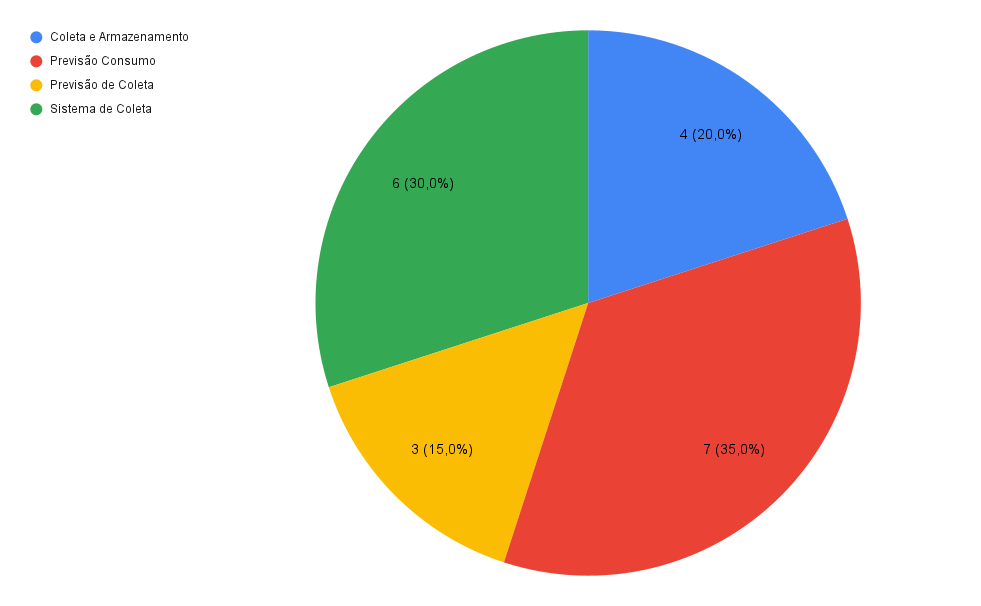
\includegraphics[width=0.8\linewidth]{Imagens/cap3/classificacao.png} 
	
	Fonte: elaborado pelo autor.
\end{figure}


Devido à necessidade de caracterizar as operações realizadas pelos dispositivos, há uma uniformidade quanto ao uso do termo "ciclo" (\textit{Duty-Cycle}) quando se pretende fazer referência às janelas de operação, nas quais o dispositivo realizará as atividades a que se propõe. Mesmo os trabalhos categorizados como soluções orientadas previsão  conforme visto na categorização apresentada na Figura \ref{fig:cap3:divisaodosestudos} apoiam-se na definição proposta por \citeonline{kansal_power_2007}, que trata ciclos como a referencia do tempo de duração das atividades que induzem um dispositivo à mudança de estados e, por sua vez, requerem capacidade energética (\citeonline{jaber_reducing_2017}; \citeonline{shen_energy-efficient_2019}; \citeonline{balsamo_hibernus_2016}; \citeonline{lee_energy_2018}). 

As soluções e propostas de adaptação dos ciclos podem ser categorizadas da seguinte forma: Primeiramente, destacam-se as abordagens que se concentram nos desafios relacionados à coleta de energia e, como consequência desses eventos, propõem mecanismos de controle e ajustes orientados a capacidade de coleta. Por exemplo, \citeonline{doumenis_lightweight_2022} descreve uma análise sobre o balanço energético coletado para definir a utilização energética do ciclo. Por outro lado, (\citeonline{choi_adaptive_2020}; \citeonline{balsamo_graceful_2016}; \citeonline{khairnar_discrete-rate_2015};) exploram, a partir da performance instantânea dos sistemas de coleta, a descoberta de motivadores para modelar a atuação do agente limitante, buscando ciclos com características neutro-potenciais.


Apesar de não se concentrar em uma solução especifica, \citeonline{kansal_power_2007} apresentam os conceitos fundamentais da teoria de coleta de energia, determinante para computação dirigida à energia. No estudo realizados por (\citeonline{khairnar_power_2011}; \citeonline{sudevalayam_energy_2011}) é considerada a possibilidade de incorporar um componente de armazenamento intermediário em conjunto com as analises de coleta, para definir como o agente limitante irá agir sobre os ciclos. Nesta direção, a proposta de \citeonline{yoo_dynamic_2012} busca comparar os valores de coleta e armazenamento para estimar como deverá ser o comportamento do dispositivo nos ciclos futuros.

Para \citeonline{liu_energy_2016}, a solução apresentada considera os custos de transmissão para definir o gasto energético durante os ciclos e assim decidir como operará. Em (\citeonline{ge_adaptive_2020};\citeonline{arnaiz_energy_2024}) é utilizado técnicas de aprendizado de máquina em busca de prever coleta e consumo de energia respectivamente. Ambos buscam antecipar características energéticas vindouras, bem como demandas ao passo que podem adaptar-se suavemente até alcançar patamar pretendido.

Outra abordagem encontrada é a desativação de recursos conforme necessário, como apresentado por \citeonline{shen_energy-efficient_2019}. Durante os ciclos, os dispositivos podem reduzir ou desligar o consumo energético de componentes não essenciais, entrando em modo restrito para reduzir o uso de energia e se adequar aos valores armazenados. Em (\citeonline{zhang_toward_2018}; \citeonline{gong_sleep_2022}), são utilizados os processos estatísticos como tomadores de decisão, baseadas em uma certa previsibilidade no fornecimento de energia e favorecido pelas características de noção do ambiente \textit{Context-Awareness} em que o dispositivo \acs{IoT} se encontra. Finalmente, a Tabela \ref{table:cap3:solucoesparajaneladeoperacoes} apresenta um resumo dos contextos nos quais o agente limitador utiliza como motivador para atuar sobre a dinâmica dos ciclos no dispositivo.


\begin{table}[H]
	\centering
	\caption{Estratégias definidoras dos ciclos de operação.}
	\small
	\rowcolors{1}{gray!10}{white}
	\begin{tabularx}{\textwidth}{|X|X|}
		\hline
		\textbf{Baseado em} &\textbf{Referência} \\
		\hline
		\multirow{6}{*}{Sistema de Coleta} & \citeonline{choi_adaptive_2020}  \\
		& \citeonline{balsamo_graceful_2016} \\
				&\citeonline{balsamo_hibernus_2016}\\
					&	\citeonline{khairnar_discrete-rate_2015} \\

		&\citeonline{benhamaid_recent_2022} \\
		&\citeonline{doumenis_lightweight_2022}\\

		\hline
		\multirow{4}{*}{Sistema de Coleta e Status Armazenamento} & \citeonline{kansal_power_2007}\\
			& \citeonline{khairnar_power_2011} \\
		&	\citeonline{sudevalayam_energy_2011} \\
		&   \citeonline{yoo_dynamic_2012}\\
		\hline
		\multirow{3}{*}{Previsão de coleta} &\citeonline{ge_adaptive_2020}\\
			&	\citeonline{zhang_toward_2018}\\
			&	\citeonline{gong_sleep_2022}\\
		\hline
		\multirow{7}{*}{Previsão de consumo} & \citeonline{arnaiz_energy_2024}\\		
			& \citeonline{lee_energy_2018}\\
			& \citeonline{luo_optimal_2017} \\
			& \citeonline{liu_energy_2016}\\
			& \citeonline{liu_performance_2015}\\
			& \citeonline{jaber_reducing_2017}\\
			& \citeonline{shen_energy-efficient_2019}\\
			\hline
		
		
		
	\end{tabularx}
	\label{table:cap3:solucoesparajaneladeoperacoes}
	
	Fonte: Elaborado pelo autor.
\end{table}

Ao analisar as características dos dispositivos \acs{IoT} que operam em restrições energéticas, a atuação dos mecanismos limitantes e as estratégias utilizadas para definir seus ciclos de operação, surge a necessidade de uma organização sistematizada dos fatores apresentados. Essa organização em formato taxonômico permite identificar e classificar os diversos aspectos que influenciam e demandam atenção na implementação do throttling, uma alternativa no processo de controle do comportamento durante os ciclos dos dispositivos.


Finalmente, a criação de taxonomia adequada possibilita uma compreensão clara das diferentes variáveis envolvidas, como características dos dispositivos, atividades realizadas, demandas de energia e estratégias de atuação do \textit{throttling}. Isso permitiria uma abordagem mais sistemática na implementação do padrão, garantindo uma gestão eficaz dos recursos energéticos o que favorece o incremento de disponibilidade enquanto conserva suas capacidades energéticas.


%\blindtext[2]

% ----------------------------------------------------------
% CAPÍTULO 4
% ----------------------------------------------------------
\addcontentsline{toc}{chapter}{Capítulo 4}
% Capítulo 4
\chapter{Taxonomia}
\label{cap:cap4}

Seguindo a análise dos trabalhos mencionados no Capítulo \ref{cap:cap3}, verifica-se a necessidade de classificar dos conceitos mais recorrentes atrelados ao uso do padrão \textit{throttling} em redes IoT com dirigidas energética. Além disso, é preciso levar em consideração a orientação do trabalho junto aos critérios de disponibilidade definidos por \cite{avizienis_basic_2004}, base para categorização dos elementos propostos nesta taxonomia. 

\section{Organização}

Inicialmente, as classes foram distribuídos acomodando os elementos envolvidos de acordo com os critérios que os definem, a seguir, conforme apresenta a Figura \ref{fig:taxonomia_geral}.


\begin{figure}[h]
\noindent\includegraphics[width=3cm]{example-image} 
\caption{Aqui vou colocar uma figura apresentando os dois grupos da taxonomia}
\label{fig:taxonomia_geral}
\centering
\end{figure}

Nas ramificações à esquerda, encontram-se categorias que representam as características principais relacionadas aos elementos presentes em ambientes \acf{IoT} com restrições significativas de energia. Em \cite{kansal_power_2007}  percebeu-se a necessidade de classificar estes elementos como pertencentes a uma relação de compartilhamento dos recursos disponíveis, sensores, atuadores e até mesmo os energéticos. Para isto, na taxonomia de \cite{avizienis_basic_2004} há uma divisão clara entre os agentes envolvidos e sua natureza em dois agrupamentos principais: um grupo denominado usuários ou clientes, que atua ativamente ou de forma passiva solicitando recursos ou quando notificado, consumindo os estados ofertados do segundo grupo, os provedores. Aos nodes provedores, cabe a responsabilidade de compartilhar seus recursos com os nodes consumidores através de uma interface conhecida de acordo com o protocolo de comunicação pré-estabelecido entre as partes.

Toda interação deve seguir um padrão de operação, esta é realizada de acordo com o qual se destina, como visto no trabalho de \cite{khairnar_discrete-rate_2015} é apresentado uma operação como a medida pelas quais mensagens são trocadas entre nodes para um determinado fim. Sendo assim, os elementos classificadores encontrados são: \textit{Agentes}, \textit{Recursos} e \textit{Operações}.

Ademais, à direita, acomoda-se os elementos envolvidos no processo de adequação do comportamento da de um node através da adoção do padrão \textit{Throttling}. Nesta, dois ramos principais são apresentados, \textit{Atuação} e \textit{Implementação} respectivamente. Sobre \textit{Atuação}, agrupa-se os elementos envolvidos no processo de controle do consumo dos recursos do node: \textit{Limiar} - \textit{Thresholding}, \textit{Ciclos de Carga} e \textit{Meios} estado diretamente relacionados à ação de limitar a taxa de resposta dos serviços,  \cite{khairnar_discrete-rate_2015}, \cite{khan_energy_2015} e \cite{sudevalayam_energy_2011} abordam questões que podem particularmente serem observadas para os elementos orientados energeticamente. A \textit{Implementação} é sugerida de maneira à assegurar que os critérios  \textit{Observáveis} e seus \textit{Motivadores} sejam agentes orientadores no processo de restrição às operações e incremento da disponibilidade do node. 


\section{Taxonomia Proposta}
A Figura apresenta em resumo a taxonomia proposta e os pontos abordados no processo de uso do padrão \textit{throttling} como alternativa para garantir disponibilidade nos nodes presentes em uma rede \acs{IoT} dirigida a energia. O objetivo principal é dispor os elementos ligados ao tema de maneira visual e contemplar a organização dos tópicos envolvidos. Com isso, obter:

\begin{enumerate}
    \item Visão sobre os elementos envolvidos em uma rede \acs{IoT} dirigida a energia e apresentar o \textit{Throttling} como mecanismo regulador do comportamento observando suas características energéticas;
    \item Organizar as classes de conhecimento relacionadas acomodando-as de acordo com o contexto de inserção;
    \item Suporte às definições de uso do padrão \textit{Throttling} ligados ao contexto de redes \acs{IoT} dirigida a energia. 
\end{enumerate}

\begin{figure}[h]
\noindent\includegraphics[width=3cm]{example-image} 
\caption{Aqui vou colocar uma figura da taxonomia proposta}
\label{fig:taxonomia_detalhada}
\centering
\end{figure}

A taxonomia detalhada apresenta suas classes nos termos em que foram encontrados na literatura dentro contexto de estudo, conforme Figura \ref{fig:taxonomia_detalhada}.

\section{Agentes \acs{IoT}}
Todo agente (node) presente é uma entidade computacional que carrega a capacidade intrínseca de interagir com outros agentes, que por definição possuem propriedades fundamentais como: funcionalidade, performance, dependabilidade e segurança como a definição já encontrada em \cite{avizienis_basic_2004}. Dado contexto, para um ambiente \acp{IoT} é fundamental considerar também a capacidade comunicar-se com outras entidades, almejando o compartilhamento de recursos \cite{li_internet_2015}, observando, além disso, suas características energéticas. 


\subsection{Node Provedor}
Qualquer entidade computacional no momento em que oferta um estado ou atende uma solicitação de recurso pode ser considerada provedor. Em geral, um provedor poderá ofertar mais de uma funcionalidade através de serviços, sendo cada uma atendida mediante o uso dos recursos durante a progressão de estados internos do provedor e seu resultado percebido como estado externo, disponível através de uma interface na forma de eventos ou a contraparte das solicitações de nodes clientes.

\noindent\includegraphics[width=3cm]{example-image} 

\subsection{Node Cliente}
Um node cliente ou usuário é a entidade que por meio de sua interface, recebe o estado externo de nodes provedores. Clientes ocasionalmente podem consumir um ou mais recursos de um mesmo provedor, mas também é possível interagir com mais de um provedor a depender da operação em execução. Enquanto cliente, o node estará interessado em realizar atividades segundo as particularidades a que se destina sua operação.

\section{Operações}
Operações consiste no fluxo de mensagens comunicáveis entre nodes clientes e provedores. Uma operação é realizada quando um cliente através de mensagens solicita estado de um provedor, de outra maneira, também é possível um provedor ativamente disponibilizar um estado, dito externo para que um possível cliente possa utiliza-lo. 

Mensagem é a unidade atômica de informação que independente do seu formato é utilizada para as mais diversas ações de acordo com o que se destina a rede colaborativa, uma mensagem pode carregar ações como  inicialização, controle, monitoramento, coleta, processamento ou armazenamento de dados. A depender da funcionalidade, um cliente quando ativo, deve enviar mensagens de solicitação aos provedores os quais reativamente respondem via interface preestabelecida, caso a operação aconteça através de eventos, o provedor deve autonomamente disponibilizará suas informações para todos que tenham interesse.

Para cobrir uma operação, múltiplas mensagens podem ser solicitadas na forma de composição de serviço \cite{service_composition}, nesse cenário um node cliente solicita mensagens distintas à um ou vários nodes provedores para compor este serviço. Em todo caso, como encontrado na revisão \cite{kahloul_service_2019} a abordagem das operações encontrada nos serviços puramente virtuais não acomodam por completo a natureza operacional dos agentes \acp{IoT}. Para tal, precisa-se considerar o estado dos nodes e seus recursos pois estes se encontram diretamente em um meio físico e precisam lidar com as particularidades inerentes a um ambiente dinâmico e seus desafios.

\section{Recursos Energéticos}

Um Recurso descreve um componente ou capacidade que um dado node possui para realizar suas operações. Isto inclui seus componentes físicos ou virtuais que uma vez embarcados ao dispositivo contribuem em cooperação para os mais diversos fins, coleta, monitoramento, automação industrial, assistência a medicina entre outros. Um Recurso infere sobre as capacidades dos elementos dispostos na rede, a configuração do dispositivo esta fortemente ligado à atividade fim que se destina. Para este trabalho, os recursos como processamento, armazenamento ou capacidade de transmissão estão omitidos pois expressam diretamente o universo de possibilidades onde um agente \acs{IoT} se encontra. Entretanto, em uma rede \acp{IoT} dirigida à energia, aspectos energéticos devem ser detalhados

Recursos energéticos refere-se a dois grupos: da capacidade de coleta do node e a capacidade de armazenamento e disponibilização da energia previamente coletada. Arquitetura de sistemas dirigidos a energia com capacidade de coleta são projetados para usar estes recursos de maneira eficiente como descrito em \cite{prauzek_energy_2018} sua aplicação é especialmente útil em cenários onde a energia para alimentar os componentes eletrônicos é escassa. Um recurso energético é propriamente uma fonte natural ou artificial de energia que de maneira apropriada pode ser convertida em energia utilizável para garantir a realização das operações. 

No cenário proposto, assume um papel importante pois é essencial para garantir o funcionamento continuo e autônomo dos nodes envolvidos, cabendo ao agente suas ações de coleta, transformar, armazenamento e utilização o recurso energético, projetado de maneira a aproximar-se do estado onde as operações tendem a uma neutralidade energética \acfp{EN}, conceito apresentado por \cite{kansal_power_2007} e mais a frente em \cite{merrett_energy-driven_2017} com a abordagem da neutralidade de força-energética, de acordo com suas respectivas capacidades.

% \subsection{Sensores}
% Um sensor é um recurso capaz de detectar e medir informações específicas do ambiente ao redor. Convertendo características do meio físico como temperatura, umidade, luz, pressão, movimento, som em sinais digitais que podem ser processados. 

% \subsection{Atuadores}
% Por sua vez, um atuador é um componente que converte um sinal de entrada em um movimento físico ou ação. Em um sistema de controle um atuador pode receber uma entrada provida por um sensor e agir em detrimento do estimulo capturado.  Atuadores geralmente são categorizados em: elétricos, hidráulicos, pneumáticos, mecânicos (por exemplo, atuadores de engrenagens), magnéticos, piezoelétricos entre outros.





\subsection{Capacidade de Coleta}
De acordo com o trabalho de \cite{sudevalayam_energy_2011}, a capacidade de coleta refere-se à habilidade do elemento em extrair e transformar um recurso energético disponível no ambiente. Seu objetivo é manter ou estender o tempo de funcionamento do node, atendendo totalmente ou parcialmente às suas necessidades energéticas.

Sistemas de coleta energética possuem três conceitos fundamentais: Carga, a Arquitetura de Coleta e entrada energética. A Carga é destinada a atividade que esta consumindo energia, este é oriundo de um componente demandante de energia para operar, sejam sensores, transmissores ou  atuadores, apresentados como uma composição de recursos. A Arquitetura de Coleta indica quais mecanismos, deve descrever seus componentes, meios de conversão e unidades de armazenamento. Atualmente é possível destacar três modelos básicos de arquitetura:

\begin{itemize}
    \item Coleta e Usa (\textit{Harvest-Use}): Neste modelo, toda energia coletada é oferecida diretamente ao node continuamente. Conforme \cite{merrett_energy-driven_2017}, um node não precisaria de um \textit{buffer} energético, ou apenas o minimo possível para mante-lo operacional, desde que seu funcionamento for orientado as características da neutralidade força-energética. Assim, a energia coletada deve satisfazer os valores de operação plena ou pelo menos o minimo necessário para o funcionamento depreciado. Por isso, caso a energia coletada não seja suficiente, o node prontamente adaptará o fornecimento dos seus recursos buscando enquadrar-se a disponibilidade energética corrente para, posteriormente, caso o nível de fornecimento energético alcance os níveis desejados, tenha sua operação restabelecida. Em alguns casos, quando prontamente é detectado níveis energéticos abaixo do necessário até para o funcionamento adaptado no node, o mesmo, poderá executar alguma rotinas de \textit{checkpoint} para caso tenha sua operação integralmente interrompida, possa mediante ter sua necessidade energética suprida em momento futuro, retornar para um estado desejado, como sistemas intermitentes já mencionados em \cite{sliper_energy-driven_2020}.
    
	\begin{figure}[h]
			\centering
			\noindent\includegraphics[width=3cm]{example-image} 
			\caption{Aqui vou colocar uma figura power-neutral}	
	\end{figure}   
    
    \item Coleta, Armazena e Usa (\textit{Harvest-Store Use}): Nesta abordagem, dispositivos inseridos em ambientes com fontes não controladas, coletam energia do meio e primariamente converte este recurso para armazena-lo em um \textit{buffer} energético daí segue disponível para carga do node, a energia armazenada pode ser utilizada como fonte secundária para adaptar a performance do node em momentos de escassez energética, o trabalho de \cite{Lee2018-iz} é um exemplo de ajustes de performance incidindo sobre o tempo de vida de nodes \ac{IoT} que coletam energia solar.
    \item Coleta, Usa e Armazena (\textit{Harvest-Use Store}): O node é alimentado diretamente pela energia coletada e transformada, todavia, em casos de abundancia energética, ou onde a energia utilizada é inferior à energia coletada, o excedente é armazenado em um dado\textit{buffer} para que em momentos de escassez ou caso exista demanda que sobreponha os valores energéticos ofertados, o node possa utilizar essa reserva como complemento garantidor dos requisitos necessários para operação.
    
    \begin{figure}[h]
    	\centering
    	\noindent\includegraphics[width=3cm]{example-image} 
    	\caption{Aqui vou colocar uma figura energy-neutral}	
   	\end{figure}  
    
\end{itemize}

\begin{figure}[h]
\noindent\includegraphics[width=3cm]{example-image} 
\caption{Aqui vou colocar uma figura com um esboço dos modelos encontrados}
\centering
\end{figure}

Diversas técnicas podem ser utilizadas para a extração de recursos, tais como a conversão de energia renovável solar e eólica, a captura da força \textit{piezo-elétrica}, entre outros. A adequação da estratégia e detalhes de coleta devem ser projetados de acordo com o meio onde node se encontra e a natureza da fonte energética que visa-se coletar. Em geral, a divisão das características dos ambientes já descrito em \cite{kansal_power_2007} é utilizada para categorizar as fontes energéticas em seus ambientes como:

\begin{itemize}

    \item Não controladas mas previsíveis: A produção energética não pode ser controlada nos momentos desejados, mas o comportamento pode ser modelado para prever a disponibilidade num dado momento com alguma margem de acerto. Por exemplo, no trabalho de  \cite{lee_energy_2018} fontes energéticas baseadas em energia energia solar, que tem sua origem não controladas, todavia existem modelos capazes de prever  disponibilidade energética para colheita de acordo com sua sazonalidade durante ciclos diurnos.
    
    \item Não controladas e não previsíveis: A fonte energética não pode ser controlada para gerar energia quando desejado e não é fácil prever usando um modelo quando será possível. A extração energética originada pela vibração de ambientes internos é um exemplo de tal fonte energética como descrito em \cite{wei_comprehensive_2017}, todavia definir padrões de sazonalidade das vibrações pode tornar o processo de coleta impraticável;
    
    \item Completamente controlada: Neste contexto, a energia é gerada apenas quando necessário, como visto em alguns sistemas \textit{piezoelétrico} onde através da interação humana para geram energia quando necessário.
    
    \item Parcialmente controlada: O processo de geração energética é sensível à ação de terceiros porém a quantidade exata de energia gerada não pode ser prevista com exatidão. Fontes baseadas em Radio Frequência converte a transmissão de ondas de radio em energia utilizável, por exemplo, \cite{shaikh_energy_2016} decorre como tags \acf{RFID} conseguem ser visualizadas por um leitor. Todavia, a quantidade de energia coletada sofre impactos diretos das características de propagação no meio disposto, barreira, distancia até a fonte e capacidade da antena de transmissão.
\end{itemize}

\subsection{Capacidade de Armazenamento}
A capacidade de armazenamento trata de propriedades como conversão, força e taxa de carregamento e descarga em relação a fonte energética em uso com o objetivo de utilizar essa energia em momento apropriado. 

É bem conhecido que o fator energético é um desafio para redes com restrições energéticas e capacidade de coleta, pois claramente caso a energia de um node seja esgotada o mesmo não será capaz de cumprir seu papel a menos que o fornecimento energético seja restabelecido ou algum mecanismo de armazenamento possa cobrir parcial ou totalmente a diferença energética necessária para a operação.

Baterias, super capacitores ou modelos híbridos estão presentes no contexto de dispositivos com fortes restrições energéticas e capacidade de coleta, para estes a atuação busca estar de acordo com as condições físicas e necessidade de conservação da energia. É possível distinguir três padrões de armazenamento para as capacidade energética presente em um dispositivo que busca o estado de operação neutra onde se observa a relação entre a saída energética e o gasto energético do node dado o momento. Segundo o modelo de uso proposto, a habilidade para coleta e a necessidade de disponibilidade definida no \acs{SLA}, os nodes provedores encontram sua capacidade de armazenamento em um dos casos:

\begin{itemize}
    \item Node provedor sem reserva energética: Aqui não existe a necessidade estrita de gestão de recursos elétricos pois caso não exista energia suficiente o node irá adaptar-se reduzindo o uso de recursos ou até mesmo interromper sua operação. \textcolor{red}{BUSCAR ALGUM TRABALHO QUE SIRVA COMO EXEMPLO.}
    
    \item Node provedor com reserva energética: Em alguns casos, um node pode se encontrar em um cenário de abundancia energética além do suficiente para sua operação, nestes, é possível incrementar os nodes com a capacidade de armazenar essa entrada energética que sobre e assim, reutiliza-la como suplemento em momento de escassez na coleta. Para tal, estes nodes devem carregar um componente \textit{buffer} energético capaz de fornecer a energia armazenada quando necessário.
    
\end{itemize}

\section{\textit{Throttling}}


A aplicação do padrão \textit{Throttling} consiste em restringir o uso de recursos através de limiares de utilização, de maneira à coibir que o comportamento de consumidores solicitantes por excessivas mensagens demandantes possam colocar em risco o funcionamento ou o dispêndio acima do esperado dos recursos do node provedor \cite{martinekuan_throttling_nodate}. A estratégia permite que provedores consigam operar dentro de seus termos definidos por um \acf{SLA}, protegendo o mesmo de assumir um estado onde precise atender mais solicitações do que sua capacidade.

 Na taxonomia apresentada, o uso de \textit{Throttling} é sugerido como adequado para colaborar as atividades que buscam aumentar a disponibilidade do node provedor, através da busca de neutralidade no uso de recursos e suas observações a respeito de suas características energéticas. Para tal, é preciso definir limiares adequados que se aplicam de acordo as regras de negócio, capacidade de transmissão e seus recursos disponíveis ou esperados no node. Definir limiares de operação realísticos para node provedor é um desafio relevante para sistemas com estratégia de coleta de energia em busca de incrementar a autonomia de atuação, observados em \cite{khairnar_discrete-rate_2015}, \cite{liu_energy_2016} e \cite{zhang_toward_2018}.

\subsection{Atuação: Limiar, Carga e Meios}
Em sistemas colaborativos orientados a capacidade energética com coleta de energia, o padrão atua gerenciando a taxa de solicitações no decorrer de um espaço de tempo em que um node cliente pode fazer requisições à um dado node provedor. Sob o ponto de vista da definição do limiar (\textit{Threshold}) de atuação, pode ser aplicado uma abordagem orientada à equidade, onde a disponibilização dos recursos por todo ciclo de vida do node provedor é constante e igualitariamente distribuído entre todos solicitantes em potencial, cabendo ao provedor apenas limitar as operações à uma mesma taxa, tolerando características que podem sofrer variação durante o ciclo de vida do node provedor, como as ligadas aos fatores energéticos de coleta e armazenamento.  Uma outra possibilidade é capacitar o node provedor para ajustar seu limiar dinamicamente, adaptando sua operação mediante as condições que se encontram. Qualquer que seja a estratégia definida deve passar pela análise cuidadosa dos recursos dos nodes  e das operações esperadas, em síntese: 

\begin{itemize}

    \item Limiar constante: o valor de limiar é fixo e estabelecido enquanto o node é projetado. Este limiar pode ser determinado considerando fatores como testes de desempenho, características do ambiente onde será inserido e requisitos operacionais. Todavia, uma vez definido, o limiar permanecerá constante ao longo do tempo de uso do node. 
    
    Por exemplo, considere um node com uma dada capacidade de processar mensagens, desprezando outros fatores como uso energético, conectividade, ou fatores de deterioração, este pode estabelecer um limiar constante para o máximo de requisições processáveis simultaneamente. Sendo assim, em toda operação, caso esse limiar de requisições seja atingido, o node irá ativamente optar por rejeitar ou atrasar o atendimento até que o valor de requisições retorne ao nível aceitado. 
    
    Esta abordagem, é bastante útil caso se conheça bem as capacidades do node e não se espera uma grande variação nas condições de operação ao longo do tempo. Embora oferte equidade do ponto de vista dos solicitantes (que tem suas requisições atendidas segundo os mesmos critérios independente do estado do node), não se garante que uso dos recursos será adequado caso ocorra  mudanças repentinas ou flutuações significativas de estado.
    
    \item Limiar adaptável: Nesta abordagem, o limiar é ajustado dinamicamente, por isso um node pode assumir um comportamento mais adequado em acordo com as condições que encontra seja através do monitoramento ou análise dos recursos do node, permitindo atender adequadamente solicitações dos nodes clientes. Por exemplo, dado um sistema de segurança que geralmente possui nodes equipados com câmeras. Os nodes, devem enviar imagens capturadas por seus sensores para solicitantes, seja uma central que passivamente recebe as gravações ou outro node demandante. Este node pode ser capaz de ajustar seu limiar de operação por fatores como numero de solicitações, largura de banda disponível, capacidade energética ou outro estado de recurso monitorado encontrado. 
    
    Graças a isso, o node com limiar adaptável alcançará diferentes faixas de operações que habilitam o node a mudar seu comportamento , ou seja para interromper ou reduzir sua taxa da transmissão e assim permanecer operando mitigando riscos funcionais. Uma vez que o recurso observável se restabeleça, o node pode assumir outro comportamento pois o seu limiar também mudará ao valor apropriado. Esta capacidade de adaptação, permite que nodes provedores mantenham algum equilíbrio entre desempenho e performance, garantindo suas funcionalidades mesmo com flutuações nas condições operacionais.
    
\end{itemize}

\begin{figure}[h]
\noindent\includegraphics[width=3cm]{example-image} 
\caption{Aqui vou colocar uma figura A e B com as diferentes atuações.}
\centering
\end{figure}


\subsection{Implementação: Observáveis e Motivadores}

A implementação deve passar por decisões arquiteturais que impactam diretamente o comportamento do node provedor bem como na eficiência de toda rede \ac{IoT}. É importante destacar que a atuação dos mecanismos de ajuste do comportamento precisam ser eficientes o bastante para que dado limiar atingido, o processo de adequação de comportamento do node provedor seja devidamente alterado, mitigando, assim, perdas desnecessárias ou não previstas, causadas por ajuste inapropriados do comportamento deste agente em questão, onde este se pode se encontrar em modo de operação fora do esperado, este modo de operação tem a capacidade de criar um cenário de esgotamento energético ou sobrecarga de atividades para outros elementos da rede colaborativa, por exemplo.

Qualquer aspecto que gere impacto ou que tenha capacidade de influenciar o comportamento neutro-energético do node com capacidade de coleta energética deve ser levado em consideração em sua implementação. Estes aspecto podem ter seus valores pré-estabelecidos, porém é comum enfrentar situações onde os valores tidos como justificadores de um comportamento não sejam suficientemente adequados, seja por uma falha na previsibilidade de um recurso ou evento não tolerável. Por exemplo, é relativamente comum um cenário onde nodes que exploram energia solar diurnalmente enfrentem alguma escassez energética motivados por eventos climáticos não previstos. Com isso, colocam em risco sua disponibilidade, pois caso seja mantido o comportamento dito adequado e previamente estabelecido podem levar o node a um alterações em sua disponibilidade não previstas ou perdas em performance. 

No contexto de dispositivos com capacidade de coleta energética, fatores pré-estabelecidos são comumente encontrados, ciclos de recarga na forma de capacidade de coleta, a capacidade de armazenamento do node e a sazonalidade da fonte energética coletável. O conjunto dos valores  desses fatores presentes no node, indicam o estado energético deste agente. Dado um estado energético esperado, pode-se previamente definir como o node se comportará. Mesmo assim, também vale ressaltar que estes elementos energéticos estão relacionados às variações e toda sorte de situações que o node provedor enfrenta enquanto agente em campo. Diversos esforços foram realizados para melhorar a maneira como um agente observa seu estado energético e define seu comportamento, mas para que seja possível adequar-se concretamente à estes fatores encontrados, o agente deve ter a capacidade de analisar as operações e o cenário onde se encontra, tanto individualmente quanto, se possível, em conjunto com outros elementos colaboradores. Assim, é possível realizar ajustes prontamente nos limiares de atuação, tão logo perceba-se que os valores estimados previamente e o seu estado esperado divirjam causando comportamento fora do desejado.

Desta forma, a mudança de comportamento do node motiva-se em: tão logo quanto os fatores de tomada de decisão forem descobertos, adequar-se para que estes fatores divergentes, aqueles descobertos em execução, sejam mitigados pois encontram-se como elementos que potencializam um risco a operação-neutra buscada pelo node ou rede colaborativa. 

No trabalho \cite{zhang_toward_2018}, equipamentos capazes estão dispostos em cenário de disponibilidade energética previsível onde é necessário em prever a quantidade futura de energia coletável disponível para recarga. O problema foi apresentado na forma de um \ac{MDP} onde os dispositivos podem adequar seu comportamento de acordo com expectativa energética vindoura para recarga.  

Por fim, na taxonomia proposta, buscar cobrir aspectos inerentes ao comportamento de operações em acordo com a neutralidade energética do node é imprescindível, a implementação das possíveis soluções que visem atender esse requisito deve observar atores estabelecidos, o contexto de uso do node, a natureza de coleta e sua finalidade ligado a capacidade e potencial de coleta para possíveis ciclos de recarga energética e por fim, sua capacidade de armazenamento, características e uso desta reserva energética.


\begin{itemize}
\item Observáveis
\item Motivadores
\end{itemize}




% \subsubsection{Valores de Operação}
% \subsubsection{Ciclos de Recarga}








% ----------------------------------------------------------
% CAPÍTULO 5
% ----------------------------------------------------------
\addcontentsline{toc}{chapter}{Capítulo 5}
% Capítulo 5
\chapter{Atividades }
\label{cap:cap5}

\blindtext[2]

% ----------------------------------------------------------
% PARTE
% ----------------------------------------------------------
%\part{Preparação da pesquisa}


% ----------------------------------------------------------
% Finaliza a parte (textual) no bookmark do PDF
% para que se inicie o bookmark na raiz
% e adiciona espaço de parte no Sumário
% ----------------------------------------------------------
\phantompart

% ----------------------------------------------------------
% ----------------------------------------------------------
% ELEMENTOS PÓS-TEXTUAIS
% ----------------------------------------------------------
% ----------------------------------------------------------
\postextual

% ----------------------------------------------------------
% Referências bibliográficas
% ----------------------------------------------------------
\bibliographystyle{abntex2-alf}
\bibliography{referencias}


% ----------------------------------------------------------
% Glossário
% ----------------------------------------------------------
%\glossary

% ----------------------------------------------------------
% Apêndices
% ----------------------------------------------------------
%% ---
% Inicia os apêndices
% ---
\begin{apendicesenv}

% Imprime uma página indicando o início dos apêndices
\partapendices
% ----------------------------------------------------------
\chapter{Título deste apendice}
% ----------------------------------------------------------

algum texto

% ----------------------------------------------------------
\chapter{título deste apendice}
% ----------------------------------------------------------
algum texto

\end{apendicesenv}

% ----------------------------------------------------------
% Anexos
% ----------------------------------------------------------
\begin{anexosenv}

% Imprime uma página indicando o início dos anexos
\partanexos

\chapter{Titulo deste anexo}
\label{anexo:anexo_mapa}
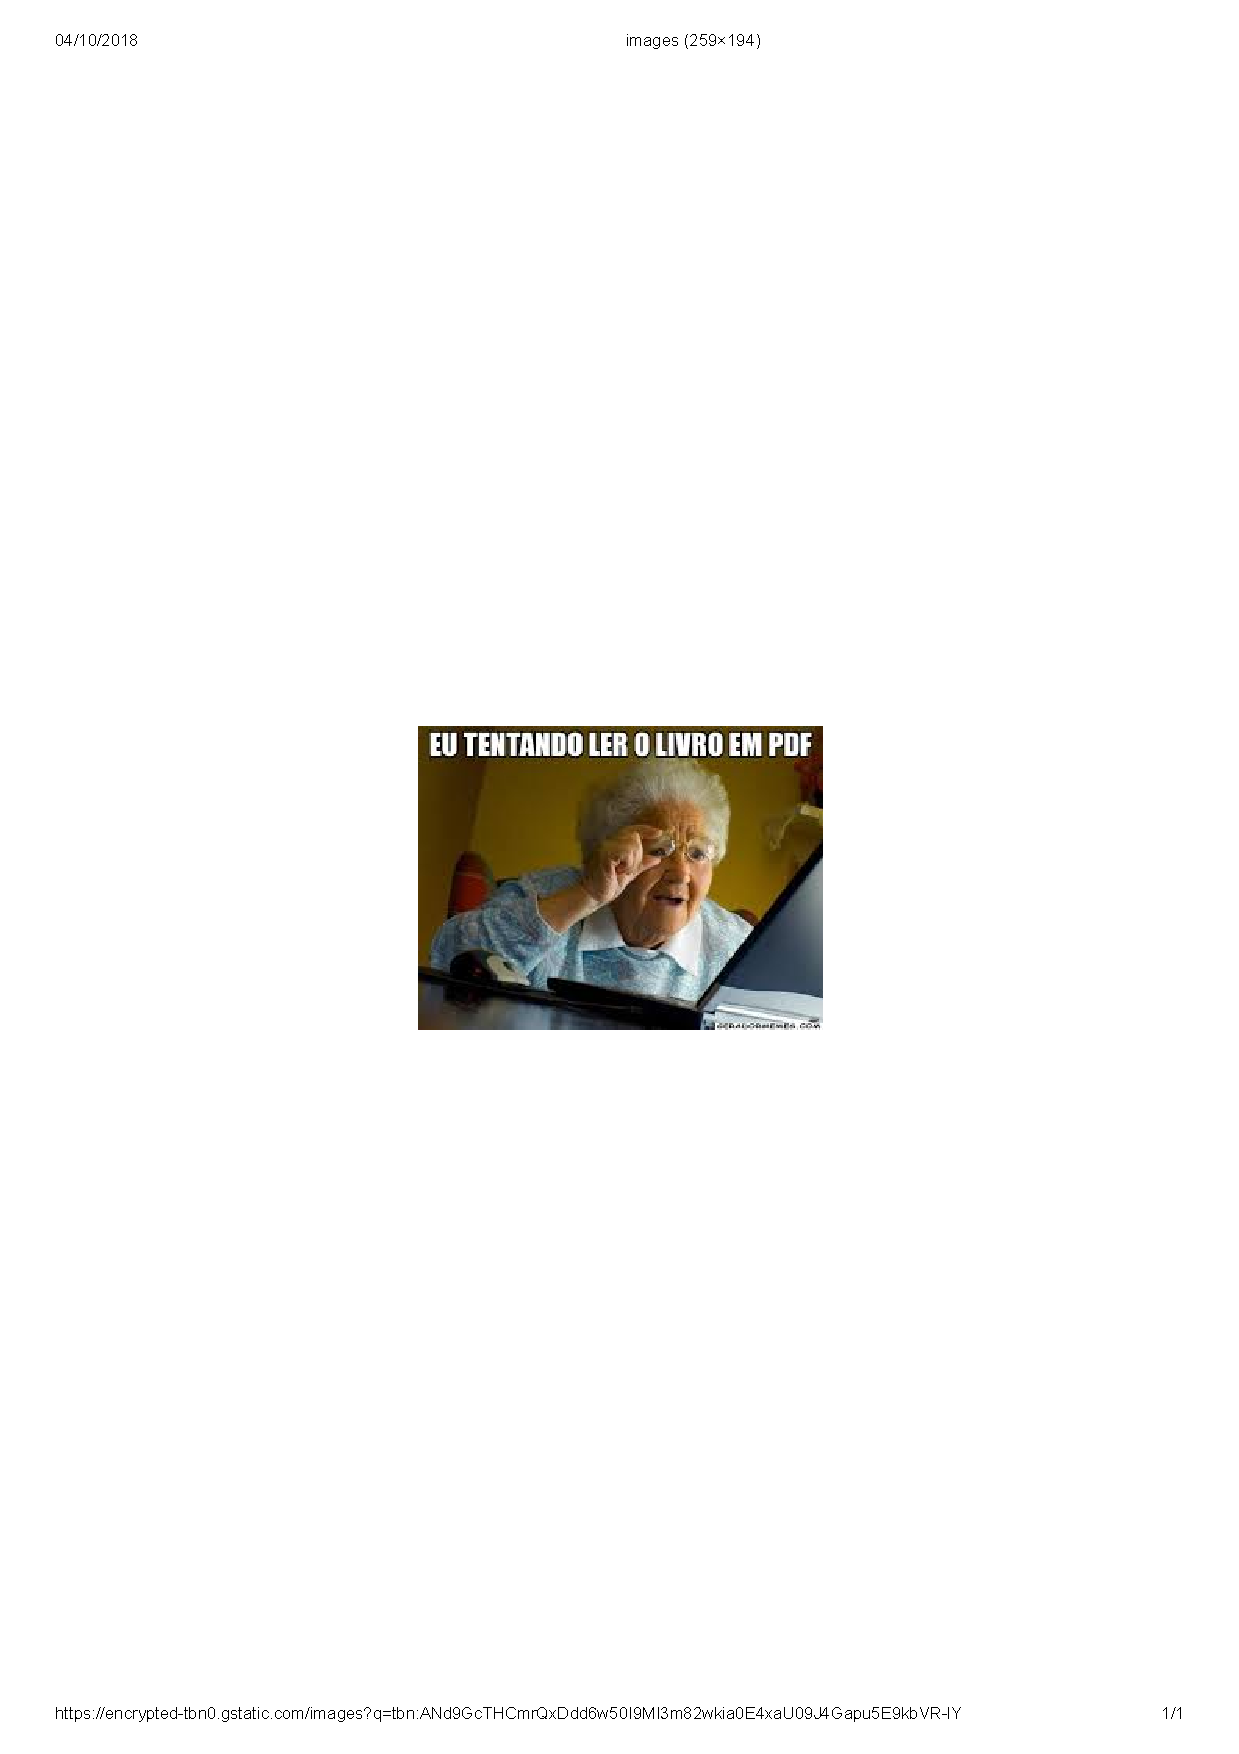
\includepdf[pages=-]{Anexos/exemplo.pdf}

\end{anexosenv}


%---------------------------------------------------------------------
% INDICE REMISSIVO
%---------------------------------------------------------------------

\phantompart
\printindex
%---------------------------------------------------------------------

\end{document}
